\documentclass{bmcart}

\usepackage{graphicx}
\usepackage{epsfig,epstopdf}
\usepackage{amssymb,amsmath}
\usepackage{flushend}
\usepackage{url}
\usepackage{caption,subcaption}
%\usepackage{hyperref}
\usepackage{fancyhdr}
\usepackage{lipsum}
\usepackage{multirow}
\usepackage{hhline,tabularx}
%\usepackage{slashbox}
\usepackage{algorithm}
\usepackage{algorithmic}
\usepackage{tikz}


\usepackage[utf8]{inputenc} %unicode support

\def\includegraphic{}
\def\includegraphics{}



%%% Put your definitions there:
\startlocaldefs
\endlocaldefs


%%% Begin ...
\begin{document}


\begin{frontmatter}

\begin{fmbox}
\dochead{NLP Term Report}



\title{Natural Language Processing}

%%%%%%%%%%%%%%%%%%%%%%%%%%%%%%%%%%%%%%%%%%%%%%
%%                                          %%
%% Enter the authors here                   %%
%%                                          %%
%% Specify information, if available,       %%
%% in the form:                             %%
%%   <key>={<id1>,<id2>}                    %%
%%   <key>=                                 %%
%% Comment or delete the keys which are     %%
%% not used. Repeat \author command as much %%
%% as required.                             %%
%%                                          %%
%%%%%%%%%%%%%%%%%%%%%%%%%%%%%%%%%%%%%%%%%%%%%%

\author[
   addressref={Cse Dept},                   % id's of addresses, e.g. {aff1,aff2}
   corref={aff1},                       % id of corresponding address, if any
   noteref={n1},                        % id's of article notes, if any
   email={cs15d006@cse.iitm.ac.in}   % email address
]{\inits{MSS}\fnm{Saranya M S (CS15D006)} \snm{}}

%%%%%%%%%%%%%%%%%%%%%%%%%%%%%%%%%%%%%%%%%%%%%%
%%                                          %%
%% Enter the authors' addresses here        %%
%%                                          %%
%% Repeat \address commands as much as      %%
%% required.                                %%
%%                                          %%
%%%%%%%%%%%%%%%%%%%%%%%%%%%%%%%%%%%%%%%%%%%%%%

\address[id=aff1]{%                           % unique id
  \orgname{Department of CSE}, % university, etc
  \street{IITM},                     %
  %\postcode{}                                % post or zip code
  \city{Chennai},                              % city
  \cny{India}                                    % country
}

\address[id=aff2]{%                           % unique id
  \orgname{Department of CSE}, % university, etc
  \street{IITM},                     %
  %\postcode{}                                % post or zip code
  \city{Chennai},                              % city
  \cny{India}                                    % country
}
%%%%%%%%%%%%%%%%%%%%%%%%%%%%%%%%%%%%%%%%%%%%%%
%%                                          %%
%% Enter short notes here                   %%
%%                                          %%
%% Short notes will be after addresses      %%
%% on first page.                           %%
%%                                          %%
%%%%%%%%%%%%%%%%%%%%%%%%%%%%%%%%%%%%%%%%%%%%%%

\begin{artnotes}
%\note{Sample of title note}     % note to the article
\note[id=n1]{Single contributor} % note, connected to author
\end{artnotes}
\end{fmbox} % comment this for two column layout

\tableofcontents
%%%%%%%%%%%%%%%%%%%%%%%%%%%%%%%%%%%%%%%%%%%%%%
%%                                          %%
%% The Abstract begins here                 %%
%%                                          %%
%% Please refer to the Instructions for     %%
%% authors on http://www.biomedcentral.com  %%
%% and include the section headings         %%
%% accordingly for your article type.       %%
%%                                          %%
%%%%%%%%%%%%%%%%%%%%%%%%%%%%%%%%%%%%%%%%%%%%%%

%\begin{abstractbox}
%
%\begin{abstract} % abstract
%\parttitle{Introduction to NLP} %if any
%
%
%\parttitle{Second part title} %if any
%
%
%\end{abstract}

%%%%%%%%%%%%%%%%%%%%%%%%%%%%%%%%%%%%%%%%%%%%%%
%%                                          %%
%% The keywords begin here                  %%
%%                                          %%
%% Put each keyword in separate \kwd{}.     %%
%%                                          %%
%%%%%%%%%%%%%%%%%%%%%%%%%%%%%%%%%%%%%%%%%%%%%%

%\begin{keyword}
%\kwd{NLP}
%\kwd{overview}
%\end{keyword}

% MSC classifications codes, if any
%\begin{keyword}[class=AMS]
%\kwd[Primary ]{}
%\kwd{}
%\kwd[; secondary ]{}
%\end{keyword}

%\end{abstractbox}
%
%\end{fmbox}% uncomment this for twcolumn layout

\end{frontmatter}

%%%%%%%%%%%%%%%%%%%%%%%%%%%%%%%%%%%%%%%%%%%%%%
%%                                          %%
%% The Main Body begins here                %%
%%                                          %%
%% Please refer to the instructions for     %%
%% authors on:                              %%
%% http://www.biomedcentral.com/info/authors%%
%% and include the section headings         %%
%% accordingly for your article type.       %%
%%                                          %%
%% See the Results and Discussion section   %%
%% for details on how to create sub-sections%%
%%                                          %%
%% use \cite{...} to cite references        %%
%%  \cite{koon} and                         %%
%%  \cite{oreg,khar,zvai,xjon,schn,pond}    %%
%%  \nocite{smith,marg,hunn,advi,koha,mouse}%%
%%                                          %%
%%%%%%%%%%%%%%%%%%%%%%%%%%%%%%%%%%%%%%%%%%%%%%

%%%%%%%%%%%%%%%%%%%%%%%%% start of article main body
% <put your article body there>

%%%%%%%%%%%%%%%%
%% Background %%
%%
\newpage

\begin{center}
\huge {\bf Chapter 1}
\end{center}
\section{Overview of NLP}
\label{sec:overview}
Languages born when human tried to communicate more information that can be 
conveyed by their sign languages and sounds. The languages evolve over a period of
time. Though the vocabulary size of a language increases, the basic unit of sounds 
(phonemes) produced to form those vocabulary are confined. The basic unit of speech is 
called phones. The set of phones confined to a language is called phonemes. Once humans
start to civilize and think, he analyzed the nature and started to discover the science
behind everything. His quest did not stop at the understanding, he also tried to apply
it in his day to day life. 

This analyzing quest turned towards the language which is the basic mode of communication when he tried to make the system to understand the same. During 1950's this natural language processing starts to get more attention as it intersected with the another vast domain called artificial intelligence (AI). 

The natural languages are very vast and un-restrictive in nature with many ambiguities This makes it tougher to come up some set of hand-written rules to feed to the systems. 
Two main problems that are needed to be faced while using hand-crafted rules are \cite{nlpIntro},

\begin{itemize}
\item Extracting meaning from the text (semantics) is hard. 
\item Hard to get even the hand-written rules to come up with human comprehensible,
'ungrammatical' phrases.
\end{itemize}

In recent years, the real time applications like 
\begin{itemize}
\item Language Translation:  translating the sentence from one language to the other, 
\item Language Identification: identifying a language from the speech, or from text,
\item Voice commanding machines: detecting or understanding the emotion or context,
\item Context based spell checking, etc
\end{itemize}
makes the natural language processing (NLP) a rigorous research field. NLP deals with text. We can describe NLP as the process of understanding and producing the understandable texts in any human language either as text or speech.  

The NLP can be split into two components namely natural language understanding (NLU) and natural language generation (NLG) as shown in Figure \ref{fig:nlpComponents}

\begin{figure}
	\begin{minipage}{0.5\textwidth}
		\centering
		\epsfig{figure=figures/nlp.eps,width=.7\textwidth}
		\caption{Components of NLP}
		\label{fig:nlpComponents}
	\end{minipage}
	\begin{minipage}{0.5\textwidth}
		\centering
		\vspace{0.5cm}
		\epsfig{figure=figures/nlu.eps,width=.75\textwidth}
		\caption{Natural language understanding}
		\label{fig:nlu}
	\end{minipage}%
		\begin{minipage}{0.5\textwidth}
		\centering
		\vspace{0.5cm}
		\epsfig{figure=figures/nlg.eps,width=.75\textwidth}
		\caption{Natural language generation}
		\label{fig:nlg}
	\end{minipage}
\end{figure}

The NLU is the process of interpreting a text and converting it into some symbolic representation for machine understanding and usage. The NLG is the process of taking some source or representation like discourse model of a language and generating a text or speech or embodied part of a document. Few examples for existing NLG are 
\begin{itemize}
\item Traffic mapping: Interpreting the satellite road maps and giving voice instructions accordingly.
\item Language translation: Converting text from one language to the other like {\textit Google translator}
\item Text to speech (speech synthesis) or speech to text conversion (speech recognition)
\end{itemize}

\section{System Vs Human Intelligence}
\label{sec:sysVshuman}

The general assumption is that NLU is harder problem than NLG. Because NLG does not require much precision as NLU. For example, one can compare automated flight take model as the NLG model where the choices and corresponding situations can be given in prior. It has to select one among the existing choices in according to the situation.
But NLU is like trying to automate the aircraft landing where many unexpected situations can appear due to the evolving nature of a language.

Another reason for NLU is the ambiguity in the source. The text which serves as the source for the NLU component, exists in both structured and unstructured ways. Humans 
do interpretation even from unstructured form of resources due to the complicated 
and still unexplored nervous system. Expecting the same from system is nearly impossible until we find out a way to interpret all those stuffs. Interpreting those information are even hard to humans because {\bf "we do many stuffs but do not know how it is being done?"}. This is because of the {\bf non-conscious} knowledge in our mind. It is hard to represent something clearly without much understanding. And to make the systems work on it, it requires more precision as discussed before. 

\begin{figure}
		\centering
		\vspace{0.5cm}
		\epsfig{figure=figures/iceberg.eps,width=.5\textwidth}
		\caption{Conscious vs non-conscious knowledge}
		\label{fig:nlg}
\end{figure}


\subsection{Structure Function Correspondence}
\label{ssec:sfcorrespondence}

The human thinking can be related to a black box, where the input is fed and output is obtained without bothering much about its internal functionality. But machines need a sequence of steps which converts the input to an output. The process is well structured.
For the successful modelling of a scenario via a machine, the whole process has to be
structured well. The modelling will be successful if the structure function correspondence is high. To be more clear, the way in which the human brain reads a newspaper by selecting the required column or section out of all the paper and interpreting the information can be considered as a function. But the same is not so simple with the system. Making the machine to understand the semantics of a phrase is a harder problem. It requires the information to be in a more structured form like tables.

\subsection{Model Diagnosis}
\label{ssec:modeldiagnosis}
The other main problem in the structure in structure-function correspondence is {\bf "notion of a structure is not universal"}. It is based on the application and its context. The system model of a scenario need not to be perfect in its first attempt. The structure of the model can be updated iteratively by observing how far its behaviour is deviating from the empirical behaviour. The model is the abstract behaviour of the system and it can be incomplete. Given the observation of a system (real-time), the model simulates the behaviour of the system. The actual observations and predicted observations are compared to understand how far the model has deviated from the system as in~\ref{fig:sysDiagnosis}. 

\begin{figure}[h]
	\centering
	\epsfig{figure=figures/modelDiagnosis.eps,width=.75\textwidth}
	\caption{Model Diagnosis}
	\label{fig:sysDiagnosis}
\end{figure}

Classical artificial intelligence (AI) can be used for better modelling of a system. The model of a system is developed by certain rules. The rule based systems may not be perfect due to certain level of uncertainty prevailing in the structure. In such cases 
{\textit "rules are padded with certain probabilities"}. The two ways in structuring a
model are 
\begin{itemize}
\item bottom-up-representation: the models are formulated from set of rules.
\item top-down-representation: first model is formulated, then rules are derived from the models.
\end{itemize}

Top down approach ensures that one is much aware of what is needed and what is to be done in a much promising way.

\subsection{Classical AI}
\label{ssec:cAI}

The study of understanding the intelligent entities of human and an attempt to represent/model it, is called artificial intelligence (AI) \cite{russelNorwig}.
AI helps to learn about ourselves and our thinking process. AI tries to address the functionality of a tiny brain. AI turned the philosophers study on how the inputs of sense organs are being remembered by this little brain into real experimental and theoretical discipline. The two broad sub-fields of AI are
\begin{itemize}
\item General purpose: logical reasoning, perception etc
\item Application specific: chess games, poetry, disease diagnosis etc
\end{itemize}

Over the decades, many definitions have been evolved to describe AI. Though there are many definitions they vary in only two dimensions namely "reasoning" and "behaviour".

\begin{table}[h]
\centering
\begin{tabular}{|c|c|c|}
\hline
%\backslashbox{Acts}{Thinks}	 & Rationally & like Humans \\ \hline
{Acts}/{Thinks}	 & Rationally & like Humans \\ \hline
\multirow{2}{*}{Rationally}  & Act rationally \& & Act rationally \& \\
							& think rationally & think like human  \\ \hline
\multirow{2}{*}{like Humans}  & Act like human \& & Act like human \& \\
							& think rationally & think like human  \\ \hline							
\end{tabular}
\end{table}

The definitions are based on \textit{"human"} performance and ideal concept of \textit{" intelligence"} called as \textit{"rationality"}. A human-centered approach is an empirical science with lot os hypothesis and experimental confirmation, while the rationalist approach is defined by the combination of mathematics and engineering. 

\subsection{AI system and Conventional system}
\label{ssec:ai-and-normal-sys}

The fundamental difference between the normal conventional system and AI system is \textbf{decision making}. In conventional system the process of decision making is encoded completely in prior with all possibilities and appropriate decisions at every possible conditions. Eg:- tree parsing

On the other hand, in AI system \textit{"what to do"} is specified but {\textit "how to do"} is not specified. That decision is to be made by the AI system. 

\section{Applications of NLP}
\label{sec:appl}
NLP is the field that deals with most of our day-to-day life products like emails, web pages, tweets, social media, newspapers, scientific articles in many languages across the world. It has the unavoidable usage right from spell check, grammar check to language translation, toy applications like automatic question answer , text comprehension etc. 

\textbf{Information extraction:} Reading a mail or passage identifying the information like date, place and create a calendar entry automatically. 

\textbf{Sentiment analysis:} Getting user feelings from the comments given for a product online. For example, when the consumer page of a camera which has lots of comments by various users about the products, analysing and splitting it into good and bad reviews can be done by sentiment analysis. 

\textbf{Machine translation:} Converting a text from one language to another language. The best and simpler example for this is the \textit{"google translator"}. Though it does not work upto the mark for some uncommon words or vernacular speech.

\textbf{Text summarization:} This produce abstract version of a document with user specific relevant information. Eg: Reading a documnet and producing the headlines, summary, outline etc. This summarization can be done on multiple documents also where a gist of the documents, or the stories that are common across the documents, or identifying the set of web pages with same content can be retrieved.

\textbf{Parsing:} Parsing is the process of representing a sentence in the form of a tree represented by the parts of speech of that sentence. Using grammar and parts of speech for parsing is a poor idea. As the grammar structure increases, the parsing tree structure will grow exponentially. If we restrict the grammar to control the parse structure it reduces the robustness nature of it. \textit{Penn's tree bank} came with an idea of annotated parsing which reduces the complication of parsing by using annotated parse tree. The annotated parse tree contains the information of parts of speech , frequency of the words, and the distributional information. 

\textbf{IBM Watson System:} This is a \textit{"question-answer"} system, based on cognitive computing. It behaves like humans by observing the data fed to it, evaluating the data based on grammar and huge set of rules programmed into it followed by decision making. Do not need structured data. It can understand from unstructured data like blogs, newspapers, websites etc. Watson does not simply looks for a synonym or keywords alone as he search engines. 	It interprets the text like a person by breaking the sentence grammatically, relationally and structurally by understanding the context. Watson performs corpus collection which is overlooked by human to remove anything that is out of date. This process is called as "curating the content". The data is preprocessed and an analogy graph is created. Training is done with the help of machine learning to understand the human interpretation via question answer pairs. Watson keeps on reading in every Q\&A process. 

\textbf{Synchronize-3-application:} This applicationalso called as \textit{"applink"}, allows the consumer's smart phones to synchronize with the vehicles thereby giving access to their smart phones seamlessly. Once synchronization is done, the user can utilize the smart phone completely in a hands free conversation mode while driving the vehicle. 

\textbf{Ring (reads text for blind):} This is an innovative invention of a ring which can be worn on a finger to read the text on a page or book. This will be very useful for the blind people as it converts text to speech.

\section{Critics of NLP in history}
\label{sec:critics}
The specific branch of AI that deals with natural language processing is called computational linguistics. The work of Norwig on computational logic is criticized by Chomsky as \textit{"a method of doing linguistics without involving language and linguistic science"}. But Norwig comments on Chomsky's work by saying it as a "notorious work in linguistics without any special regard for real-data. Chomsky wants to represent language with elegant theory which clearly surpasses the human erroneous nature and to get the simple structure lying under his complex brain structure. Meanwhile Norwig tries to represent everything by simplistic statistics. Chomsky commented on the statistical machine learning methods that mimics the behaviour of some real world scenarios, as to simulate the bee dance without understanding the reason behind that dance. But Norvig claims that why should we complicate the process instead of following statistical model which is simpler and efficient. Norwig argues that every word in a language occurs with certain frequency and that frequency can be learned from the humongous amount of data.


\section{Morphology}
\label{sec:morphology}

The source of NLP is "TEXT". The basic element of text is character. A sequence of character giving a proper meaning is called as a word. The sequence of words forming conveying an information is called sentence. Sentences together form the paragraph also know as discourse. This structure can be linked with chemistry and it looks like the Figure~\ref{fig:morphology}.

\begin{figure}[h!tb]
\centering
\begin{minipage}{0.5\textwidth}
	\centering
	\epsfig{figure=figures/morphology.eps,width=.5\textwidth}
	\caption{Morphology}
	\label{fig:morphology}
\end{minipage}%
\begin{minipage}{0.5\textwidth}
	\centering
	\epsfig{figure=figures/word_language.eps,width=.75\textwidth}
	\caption{Words-Language relationship}
	\label{fig:morphology}
\end{minipage}
\end{figure}

The characters are similar to electrons which are the basic elements and do not convey any meaning when it is used alone. The combination of electrons leads to atoms and atoms are bonded to get a valid molecule. The combination is determined by the valency bond. Similarly the combination of words to make a meaningful sentence is determined by grammar and structure of the language. 

The words evolve over a period of time. One word can be used to form the other by many process like \textit{derivation} (Eg: educate --> education), \textit{inflexion} (sing --> singing), etc. When words used in sentence, the role of it in the sentence is determined by \textit{parts of speech}. The meaning of two individual words change completely when they come together. \textit{Eg: ice-cream, honeymoon, pass-away ...}

Lexical analysis comes into picture in the formation of words from characters and semantics comes in to picture when words are combined to form a sentence. Sentences together form a paragraph or passage. Analysis the paragraph is totally a different task known as \textit{discourse analysis}.

	Words evolve over a period of word, which leads to higher dimensionality problem when documents are processed on word basis. As the words of a language increases it is not necessary for the language also to grow in same rate. This is because, all the words in  the language are not used in daily interactions or in all context base don the life-style. Thus the growth of words of  language an d the language are non-linearly related. 
		
	
\subsection{Word Co-occurrence}
\label{ssec:co-occurrence}

The relation between two words is defined as word co-occurrences if both words are in association with each other in some sense. That is, if there is a document with a word heart surgery, it is more likely to find the word by-pass surgery or angiography in the same document. If the related word are found in same document, then they are referred to
as \textit{"first order co-occurrences"}. If the related works are found in two different documents then they are called as \textit{"second order co-occurrences"}.


\subsection{Ambiguity and its types}
\label{ssec:ambiguity}

	Analysing and understanding a text/speech segment is pretty tough for a machine. 
Humans understand it duet to the cognitive knowledge that acts as a very big database formed right from one's child hood. When some one asks you \textit{Is there water in jug?} it means if the water is there we have to pass that jug to the person who asked that question. Such sentences are called {\bf pragmatics}. But system will not understand pragmatics. The process of understanding a word in more than one way is referred to as \textbf{ambiguity}.  Ambiguity can occur at various levels of NLP. Ambiguity could be Lexical, Syntactic, Semantic etc \cite{ambiguity}. 

\begin{itemize}
\item {\bf Syntactic ambiguity:} This ambiguity involves operators and quantifiers. 
{\textit Eg: {Every man loves a woman}}. Here there are two kinds of interpretations. The one is "For every man there is a woman", and the other is "there is one particular woman who is loved by every man". The scope of quantifiers are not clear and it can create ambiguity.
\item {\bf Semantic ambiguity:} This occurs when the meaning of the word itself is interpreted in more than one ways.\textit{ Eg: We saw her duck}. Duck can refer to the
person’s bird or to a motion he made. Semantic ambiguity happens when a sentence contains an ambiguous word or phrase.
\item {\bf Discourse analysis:} This analysis gives the information about the influence and relationship of across the sentences.This analysis includes \textit{(i)Co-reference resolution} and \textit{(ii) information extraction}. Co-reference identifies the  phrases in a document that refers to same information. Information extraction locates specific piece of data from a document. 
\end{itemize}

\section{Types of Knowledge}
\label{sec:knowledgeTypes}

Humans infer the language through the knowledge they acquire from there childhood \cite{childknowledge}. The process of a child getting the worldly knowledge from its care-takers and surroundings is termed as \textbf{"child knowledge acquisition}. Similar to this knowledge source, system needs knowledge to process the natural language. The knowledge that contributes the database for NLP can be divided into three types namely
\begin{itemize}
\item \textbf{Linguistic knowledge:} The dictionary is an example for linguistic knowledge from where one can get the common knowledge about the use of language. Explanations, meanings and synonyms of a word and their usage helps us in understanding
the language in a proper way. \textit{Eg: Oxford dictionary}

\item \textbf{Introspective knowledge:} The knowledge within the given documents or reports are considered as introspective knowledge. The information like co-occurrences of words at different order (statistical co-occurrences) constitutes the introspective knowledge. 

\item \textbf{External knowledge:}The world knowledge or external knowledge can be divided under variety of various fields. This knowledge also includes the common information shared across the fields also. The effective representation of knowledge via human media such as pictures, diagrams, voice, knowledge drawn from textbooks, encyclopedia, glossaries etc. 
\textit{Eg: Wikipedia}
\end{itemize}

\section{Linguistic processing}
\label{sec:languageProcessing}

\begin{figure}
	\centering
	\epsfig{figure=figures/knowledge.eps,width=.5\textwidth}
	\caption{Shallow and deep linguistic analysis}
	\label{fig:morphology}
\end{figure}

Language processing needs theoretical and descriptive analysis. Based on the level of analysis the linguistic processing is classified into (i) deep and (ii) shallow processing. 
\begin{itemize}
\item \textbf{Shallow linguistic processing (SLP):} SLP also known as machine learning approaches altered the fundamental processing of NLP. Many rapid and robust creation of tools have been developed for this SLP which requires lesser time and manual effort. So the SLP gained more interest than deep linguistic processing. This can also be termed as \textit{knowledge light NLP}. 
\item \textbf{Deep linguistic processing (DLP):} DLP is concerned with more computational development. The grammars for DLP were manually developed maintained and are computationally expensive. But the cost can be trade off with the effective performance given by DLP than SLP. 
\end{itemize}

\newpage
\begin{center}
\huge {\bf Chapter 2}
\end{center}

\section{History of NLP}
\label{sec:history}
In 1948  the first NLP application was developed for searching a word in dictionary using a look-up system. In 1950 the first machine translation was implemented to translate Russian language to English. The NLP really took its intense phase of growth from 1957 after the syntactic structures proposed by Noam Chomsky. Many researches are started after that and still evolving. After the introduction of machine learning and artificial intelligence the research development in NLP took a vertical growth.

The unavoidable usage of internet and technologies, made NLP as an essential part of peoples every day life. Chatter-bots like PARRY, Recter, and Jabberwacky were written and developed during early times of NLP research. The IBM Watson discussed in Section~\ref{sec:appl} was invented in 2011 which is a question and answer (Q\&A) application, which makes the user so transparent to the system that responds from the other end. It is a general purpose artificial intelligence based system, which can hold a human-level conversation. 

An enormous quantity of preprogrammed knowledge concerning both the language and the domain under examination is the prerequisite of any natural language processing application. 
The increase in computer power made this transformation possible thereby allowing more research and programs to be written for NLP.

\section{Why NLP is hard?}
\label{sec:hardNLP}

Sheer complexity of sentence structure of our text/spoken language makes the NLP problem harder to get implemented. The indicatives also known as \textit{known facts}, and our rationally questioning nature of \textit{"what if...?} in many cases increases complexity in formulating the rules for these kind of applications. Processing text in becoming more hard because of the various methods of formulating the text. For example it is rule to use periods (.) after the title like \textit{Mr., Mrs.,} etc and at the end of the sentences. its is harder to find and differentiate between these two periods, wherein other unnecessary and unwanted periods are being inserted in many places due to lack of awareness which makes the \textbf{sentence boundary detection} problem more complicated. 

Apart from the lack of common notation in writing a text information, the syntactic ambiguity because of the polysemous words makes it tough to understand and differentiate the words. The major and still unsolved problem is the context detection in the language. The meaning of the sentences vary depending on the intent of the speaker, listener, location, prior, time and social content as shown in some scenarios given below~\cite{nlpHard}.

\begin{itemize}
\item     Depends on the people present e.g. "How far is it?" (miles or km)
\item     Depends on the social context: "That was bad!"
\item    Depends on the location, e.g. "It is playing in upstairs" (It refers to song that is being played in upstairs.)
\item     Depends on the time of day, e.g. "Let's go eat" (eat may refer to breakfast, lunch or dinner)
\item     Depends on prior sentences: "The third one" (depends on what other two are?)
\end{itemize}

Apart from this, recognising the names of people, place, animal, object and differentiating the various slangs, jargon, sarcasm, spelling mistakes, humour, grammar mistakes etc makes the natural language processing the more challenging research problem. 

\section{Artificial Intelligence}
\label{sec:AI}
Artificial intelligence can be literally defined as the intelligence possessed by machines or software. 	AI is the separate engineering field where the study deals with making intelligible machines and software. Intelligence in here describes the ability of the system that perceives the environment and takes the action such that it maximizes the chance of success in whatever application it work towards. AI has its own part from generalized applications to specific applications like gaming. The AI is used where there is the need for reasoning, planning and learning. Since NLP has all these in its field, AI is used widely in NLP. Humans have the ability to precisely describe their need and making the system to simulate it. But the range of precision clearly affects the performance of the system. As far as the rules are clear, systems will work fine with it.

AI leads to many latest and admirable inventions like smart phones, automatic vehicles, smart homes, auto-bots, language learning tools, hardware interactions etc. Many IVR based systems are developed for ubiquitous interaction of humans with the machines and electronics on the fly. This is made possible only because of the fusion of two most important and complicated fields by thte name AI nad NLP.

\section{Conscious and non-conscious Knowledge}
\label{sec:knowledge} 

Right from the child hood we humans do many task with the help of our organs controlled by the only CPU in our head called brain. The tasks like understanding a language, picking up the required sound from crowded hall, summarizing the text document, inferring the image and storing the details, everything are done just like that without much knowledge of "actually how it is done?". These actions are done as an involuntary reaction for the instructions given by the brain. If we decode these set of actions and understand it, then it will be easier for us to instruct the machines to follow the same set of instructions to simulate the human behaviour.

But it is hard to explain something that one does not understand black and white. Those unexplainable knowledge is termed as \textit{"non-conscious-knowledge"}. If one can able to answer a question clearly by description or diagram or by any means the same can be interpreted by system if the way of our interpretation is given to it as input. For example, if some one asks to define force, it can be defined empirically and mathematically. This is because of \textit{conscious knowledge} which we obtain through our rational understanding. If someone asks to explain a color, it is impossible to explain unless one see many object with same color and classifies it internally with that class label "green". This happens because of the \textit{non-conscious} knowledge that resides in our brain due to the humongous processed database collected right from our childhood.

\newpage
\section{Morphology}
\label{sec:morpho}
The smallest meaningful grammatical unit in a language is called \textit{morpheme}. The study of morpheme sis called morphology. 	The morpheme and words are not same. Morpheme may or may not stand alone. But words always stand-alone~\cite{morphology}.
There are different types of morphemes as described below:
\begin{itemize}
\item {\bf Free morphemes:} The morphemes that are stand alone and act as words. Eg: dog, cat, town, city etc.
\item {\bf Bound morphemes:} Appears as a part of a word. Always occurs in conjunction with a root word as affixes, prefixes, and suffixes(tion, ing, ation etc). 
\item {\bf Derivational morphemes:} The morpheme together with the standalone word called as root word, changes the meaning or parts of speech of that root word. \textit{Eg: happy+ness=happiness. Happy (adjective), happiness(noun)}.
\item {\bf Inflectional morphemes:} Modifies the verb's tense or a noun's number without affecting the meaning. 
\textit{Eg: Sing+ing=singing. Root: sing, singing(current ongoing action).}
\end{itemize}

As discussed in Section~\ref{sec:morphology}, the character forms the basic of a written language from where the words, phrases, sentences and paragraphs are formed. In spoken language the same sequence can be compared with phonemes, syllables, words, sentences and paragraphs. Phonemes are like the basic elements. The combination of vowels (V) and consonants (C) as CV, VC, CVC, CCV, etc forms the syllables. The syllable structure of every language varies. The basic sound units of a language are termed as \textit{"phones"} and the sounds that are confined to a language are called as \textit{"phonemes"}.

The words of a language keep on evolving. The one brilliant idea followed or insisted by our ancestors are to keep the basic sound units, i.e., phonemes constant and evolving new words as per the requirement based on these phonemes. Apart from the semantic ambiguity or context difference, difference and complications starts to occur right from the word level of a language. There are different words with same meaning(synonyms), different or same spelling words with same pronunciation (homonyms), a word having more specific meaning than the other (hyponym), a metaphorical word, that used to refer the other word which actually points to the part of a whole (meronym) etc. Understanding and differentiating these words are not a trivial task.

These problems can be solved by having large number of examples for each word in the database and tagging them with descriptions called synsets. This helps us to resolve the syntactic ambiguity problem to a certain extent. 

\section{Ambiguity}
\label{sec:ambiguity}
Ambiguity in NLP occurs in all levels of analysis right from the morphology to discourse analysis. Coming up with a software that decides the meaning of a given text or speech without considering the context is like a lost battle. The basic definition of ambiguity 
can be given as \textit{"the ability to understand the piece of text/information in more than one way"}~\cite{ambiguityTypes}. The most common types of ambiguity from literature are
\begin{itemize}
\item {\bf Lexical ambiguity:} More than one interpretation of a word. Eg: Flies ( an action of flying / an insect)
\item {\bf Syntactic ambiguity:} Variation in the interpretation of a sentence due to the grammatical structure. Eg: He saw her duck ( duck may be an action/a bird).
\item {\bf Semantic ambiguity:} Different interpretations of meaning based on the based on the meaning of words in the phrase when combined. Eg: \textit{"Colourless green ideas sleep furiously"} is a sentence composed by Noam Chomsky in his book "Syntactic Structures" as an example of a grammatically correct, but semantically nonsensical statement. 
\item {\bf Pragmatic ambiguity:} The context of the phrase or sentence gives completely different meaning for the sentence's actual meaning. This commonly happens when conversation happens between two entities in different domain without any common basis. 
Eg: \textit{"superfluous hair remover"}. Here we are not sure whether the superfluous describes the process of hair remover or the noun remover. Because of the improper representation of scope of specifier this pragmatic ambiguity may occur.
\end{itemize}

\section{Child knowledge acquisition}
\label{sec:child}
Language acquisition is the process of acquiring the capacity to understand and interpret a language, and to communicate in that language. This language based communication is meant especially for homosapiens~\cite{childknowledge}. Usually the language acquisition starts right from our childhood, from the surroundings and caretakers. There are two types of language acquisition in general for a child namely (i) first language acquisition and (ii) second language acquisition. To get expertise in a language, one need to now different range of tools right from phonology, morphology to extensive vocabulary in that language. Language can be written as text or vocalized as speech. 

The general approaches of child knowledge acquisition are (i) social interaction and (ii) emergent-ism. The former one happens because of the interaction interaction of a child with the linguistic-knowledge-adults. The instructive corrections given to the kid by its care-givers helps the child to correct the language. This works as a black box with feed-back mechanism. The later one can be defined as the cognitive process that emerges by the biological pressures and environment. This can be related a=to an example for better understanding. If a person familiar with only the mother tongue is relocated to another place with completely different language, he will learn that new language quickly for his better survival in that environment. The theory of child and adult knowledge acquisition process is detailed in~\cite{childknowledge1}.

\section{Other applications of NLP}
\label{sec:nlpApps}
\begin{itemize}
\item {\bf Co-reference resolution:} This is the process of analysing the given text document or a chunk of text and identifying the words referring to same information. For examples, matching up the pronouns with the nouns that are referring to. It is also called as "bridging-relationships" 
while referring the structure of one thing in a sentence.
\textit{Eg: She peeped in to Rosy's house via the glass window.} In this sentence, the glass window is the structure of Rosy's house. It indirectly refers to Rosy's house. 
\item {\bf Morphological segmentation:} The process of identifying the morphed words, separating it from the root word and classifying the morphemes is called morphological segmentation. For few languages like English which has simple morphology, all possible words can be listed instead of going for morphological segmentation. But this is not the case in highly agglutinated languages like Tamil, Turkish etc. 
\item {\bf Named Entity Recognition (NER):} Given a stream of text, predicting the upcoming word or next word or completing the present typing the word is called NER. Forming a common way of writing the text to identify the starting of hte word will also fail in case of representing the name of a a person, place or animal. Handling this is also another difficult problem in NLP.
\item {\bf Optical Character Recognition (OCR):} Scanning text from a scanned image of a document/book. There is a problem of mis-interpreting two closely written characters. \textit{Eg: Interpreting "cl" as "d"}.
\item \textbf{Sentence boundary disambiguation:} Usually the written texts are bounded to some rules like the usage of periods and punctuations for better readability and sense. But the same can also be used to represent abbreviation. To make the difference between the sentence period and abbreviation-al notations, and segmenting the sentence accordingly is called as sentence boundary disambiguation. 
\textit{Eg: I woke up at 5 A.M. I went for a walk and met the C.E.O of a company in the park.} Here the difference between the period after 5 A.M and the punctuation between A.M and C.E.O needs to be differentiated.
\end{itemize}

\section{Summary and Conclusion}
\label{sec:conclusion}

	The Sections~\ref{sec:overview} to~\ref{sec:languageProcessing} in Chapter 1, gives the verbatim of the introduction of NLP taught in the first week classes. These chapters helped us to understand the basics and origin of NLP field and the current trending application of it. The NLP evolved when humans try to simulate the language behaviour through the system for faster and easier communication in this technological world. The mapping between the human knowledge and that of the systems (artificial intelligence) are discussed in Section~\ref{sec:sysVshuman}. The general structure of any language is learnt from morphology discussed in Section~\ref{sec:morphology}. The type of knowledge required by the system to perform any NLP tasks is elaborated in Section~\ref{sec:knowledgeTypes} and the methods of language processing by the systems is discussed in Section~\ref{sec:languageProcessing}.
	
	The remaining Sections from~\ref{sec:history} to~\ref{sec:nlpApps} discusses the information I gained through the self-study suggested during class hours. Section~\ref{sec:history} is just the output of a curiosity in digging the origin of NLP and its evolution in the current trend. Section~\ref{sec:hardNLP} is the suggestion for defining natural language processing as a hard problem. Section~\ref{sec:AI},~\ref{sec:knowledge} and~\ref{sec:ambiguity} is about my views on AI, conscious vs non-conscious knowledge and ambiguity. The term child knowledge acquisition mentioned in class and through the video lecture from TED talk made me to search and understand the process of language knowledge acquired by a child, which is explained in Section~\ref{sec:child}. Apart from the NLP applications discussed in class, few more applications are elaborated in Section~\ref{sec:nlpApps} which caught my interest.

\newpage
\begin{center}
	\huge{Chapter 3}
\end{center}

\section{Introduction}
\label{sec:takeAway}

The natural language processing as over-viewed in 	first two chapters has loads of applications in 
real-time which need to be un-earthed to reach realize it's full effectiveness in our day to day 
life. This chapter comprises of problems the cause, the symptoms and solutions of real time 
problems that are attempted and solved (in many cases) till now. From the duration of past 6 months with the help of the course instructor, I felt the following are the important take-aways that I understood and  can implement in real from the help of related published materials.

\begin{itemize}
\item Spell checking
\item Information retrieval
\item Semantic relatedness
\item Word sense disambiguation
\item Circularity problem
\item Parsing and
\item Machine translation
\end{itemize}

Each of the above enlisted topics are discussed in detail in other sections of this subject.

\section{Spell Checker}
\label{sec:SpellCheck}

Spell check is the process of identifying misspelled word in the given phrase or sentence. This
can be implemented with different granularity like
\begin{itemize}
\item word-level
\item phrase-level and
\item sentence-level.
\end{itemize}

If a word is mis-spelled we have to play with just 26 characters in different combinations to come up with correct-word \cite{spellCheckSurvey}. A word is decided as a proper word if it exist in dictionary. With this this, the spell-corrections at word-level can be done.

But in case of phrase level the other problems occurs. {\it {Whether to identify all mis-spelled
word in the phrase?} or {\it a single word} }. The other problem pops up, when the correct spelled word occurs in wrong context like {\emph{I saw her near the see / A peace of cake}} etc.

The other important requirement to perform spell check is the dictionary. This dictionary can be any kind of thesaurus, digital dictionary or a huge collection of real-time text data which can act as a repository to check with all the possible alternates for the mis-spelled word. This set of alternatives are termed as {\bf "Candidate List"}.

\subsection{Edit Distance to Generate Candidate List}
\label{ssec:editDistance}

From one word we can get another word by any one of the following process

\begin{itemize}
\item Insertion ( port $->$ sport )
\item Deletion ( Spark $->$ park )
\item Transposition ( hte $->$ the )
\item Substitution ( spine $->$ swine )
\end{itemize}

Edit distance algorithm follows the strategy of dynamic programming, where the solution of a problem depends on the solution of its sub-problem.  This nature is defined as the {\textit{optimal sub-structure}}. This algorithm also has the \textit{"overlapping sub-problem nature"} which can be illustrated by the example of Fibonacci series represented as 
\begin{equation}
Fib(n)=Fib(n-1)+Fib(n-2)
\end{equation}
The computation can be made faster by solving the sub-problem and saving the result in a look-up table which can be used for the new computations.

\subsubsection{Applications of Edit Distance Algorithm}
\label{sssec:appln_editDist}
The edit distance algorithm has its applications in different fields of science and engineering as listed below:
\begin{itemize}
\item Spell check (character level comparison)
\item Machine translation ( word level comparison)
\item Speech recognition (word level comparison)
\item Computational biology (DNA sequence comparison)
\end{itemize}

\begin{algorithm}[h!tb]
\caption{Edit distance algorithm}
\label{algo:modgd}
\begin{algorithmic}[1]

\STATE \COMMENT{\textbf{Input:} Two words $w_{1}$ and $w_{2}$\\
\textbf{Output:} Edit distance between the words}
\STATE Initial condition or base condition 
\begin{equation*}
D(i,0)=i;  \quad
D(0,j)=j;
\end{equation*}
\STATE When j $\neq 0$ or i $\neq 0$ 
\begin{equation*}
D(i,j)==min \left\{\begin{matrix}
\hspace{-3.3cm} D(i-1,j)+1 \\ 
\hspace{-3.3cm} D(i,j-1)+1 \\
D(i-1,j-1)+\left\{\begin{matrix}
1, & if \quad s_1(i) \neq s_2(j) \\ 
0, & if \quad s_1(i) = s_2(j)
\end{matrix}\right. 
\end{matrix}\right.
\end{equation*}
\end{algorithmic}
\end{algorithm}

Any one of the operations mentioned in Section~\ref{ssec:editDistance} is used with the cost associated with it. The edit distance of to words PARK and SPARKE is given in the following matrix

\begin{table}[h!tb]
\begin{tabular}{c|c|c|c|c}
    & P & A & R & K \\ \hline
 S & 1 & 2 & 3 & 4 \\ \hline
 P & 1 & 2 & 3 & 4 \\ \hline
 A & 2 & 1 & 2 & 3 \\ \hline
 R & 3 & 2 & 2 & 2 \\ \hline
 K & 4 & 3 & 3 & 3 \\  \hline
 E & 4 & 3 & 3 & 3 \\
\end{tabular}
\caption{Edit distance matrix of  two words Spark and park}
\label{tab:editDist_matrix}
\end{table}

The total edit distance of sparke and park is 3 (value in the right-most bottom cell of the matrix). The time complexity of the edit distance algorithm is $O(m\times n)$ where $m$ and $n$ are the lengths of $word \; w_1 $ and $ word \; w_2$.

\subsection{Bayesian Probability}
\label{ssec:bayesProb}
Once the candidate list of words with corresponding edit distance is obtained, then Bayesian probability as mentioned in Equation~\ref{eqn:bayes} \cite{spellCheck}. $P(C|T)$ in the Equation~\ref{eqn:bayes} is referred as $posterior$ probability calculated from $P(T|C)$, the $likelihood$ of the typo given correct word, $P(C)$ the prior of correct word from the dictionary or database, and $P(T)$, the evidence of the typos i.e, the mis-spelled word.

\begin{center}
\begin{equation}
P(C|T)=\frac{P(T|C)*P(C)}{P(T)}
\label{eqn:bayes}
\end{equation}
\end{center}

The likelihood ratio is computed by the ratio of bi-grams or tri-grams of the typo and the correct words. This can be explained with the example of two words say "acress" and "actress". The tri-gram sequence of "acress" and "actress" are,
\begin{itemize}
\item acress (T): {acr,cre,res,ess}
\item actress (C): {act,ctr,tre,res,ess}
\item $|T \cap C|$: | res,ess | = 2
\item $|T \cup C|$: | acr,cre,res,ess,act,ctr,tre| = 7
\item Likelihood term :  $P(T|C) \quad = \quad \frac{|T \cap C|}{| T \cup C|} \quad \frac{2}{7}$ 
\item  Prior term: $P(C)=\frac{n}{N}$ where $n$ is the frequency of $C$ in corpus and $N$ is the total number of words in the corpus.
\end{itemize} 

\subsubsection{Smoothing}
\label{sssec:smooth}
The major problem in calculating prior is to handle the unseen words. If a word which is no tin the database or corpus used as dictionary is encountered the whole $Posterior$ term goes to zero because of the zero prior. In order to handle this the process of smoothing is invoked. The most commonly used smoothing technique is the \textbf{Laplace Smoothing} also known as \textbf{add-one smoothing}.

	\begin{itemize}
	\item {\bf Laplace Smoothing} is the process of adding certain value to the prior of every word found from the corpus. The smoothed prior is calculated as 
	\begin{center}
	\begin{equation*}
	P(C) = \frac{n+0.5}{N+0.5V}
	\end{equation*}
	\label{eqn:laplaceSmoothing}
	\end{center}
	\end{itemize}

	The other alternate ways of smoothing also present. One such method is {\bf Good Turing Discounting}. 
	\begin{itemize}
	\item {\bf Good Turing Discounting:} Here the unseen classes are termed as {\it zero training } classes and Good Turing probability for zero training classes are calculated as
	\begin{center}
	\begin{equation}
	P_{GT} = \frac{N_1}{N}
	\end{equation}
	\label{eqn:pgt_unseen}
	\end{center}
	where $N_1$ is frequency of classes or sub-population with minimal frequency identified so far, and $N$ is the sum of all class frequencies identified so far.
	Once $P_{GT}$ is computed the probabilities of each class is re-computed as follows:
	\begin{center}
	\begin{equation}
	\hat{C} = (C+1) \frac{N_{C+1}}{N_C}
	\end{equation}
	\label{eqn:pgt-re-est}
	\vspace{-1cm}
	\begin{equation}
	P(C)=\frac{\hat{C}}{N}
	\end{equation}
	\label{eqn:pgt-new-prob}
	\end{center}
	where C refers to the class and $N_C$ refers to the frequency of class $C$.
\end{itemize}	 

The candidate word with maximum posterior is considered as the correct replacement for the mis-spelled word.

\subsection{Phrase level spell check}
\label{ssec:phraseSpellCheck}
	Edit distance is used to identify the appropriate candidate list for the mis-spelled word. Once the candidate list is generated the possible phrases are generated with all the candidate elements and the probabilities of all possible phrases along with the context are computed from the corpus as 
	\begin{equation}
	P(w|c_{-k}.c_{-k-1}.\cdots c_{-1}.c_{1}.c_{2} \cdots c_{k}) = \frac{P(c_{-k}.c_{-k-1}.\cdots c_{-1}.c_{1}.c_{2} \cdots c_{k}).P(w)}{P(c_{-k}.c_{-k-1}.\cdots c_{-1}.c_{1}.c_{2} \cdots c_{k})}
	\end{equation}
	where $C_k$ are the collocation words. Collocation words are the words located in close proximity with the considered word. But context words are the need not be close in spatial terms. It can be anywhere in the document and the it is assumed that if we find that word, it is more likely to find the other word related to that in the document.
	
	 This scenario of context based spell checking can be explained with following example.
	Eg: From the eath to the moon
	
	\begin{itemize}
	\item Candidate List: { death, earth}
	\item Possible phrases: 
		\begin{itemize}
		\item From the death to the moon
		\item From the earth to the moon
		\end{itemize}
	\item Calculate the probability of each phrase from the corpus. The phrase with maximum probability is considered as the correct phrase.
	\end{itemize}

	The other scenario is handling the $confusion$ words. Consider the example {\bf "$peace$ of cake"}.  Here though the spelling of "peace" is correct, it does not suit for the phrase. In such cases, we have to compare the phrase with the list of confusable words. All possible sentences with confusion words are formed and the sentence or phrase with maximum probability is chosen as the correct phrase as usual.
	
\section{Information Retrieval}
\label{sec:ir}
Information retrieval (IR)  can be broken  down to prior and likelihood of the documents involved.  Different formalism for information retrieval are there. A non-probabilistic approach for information retrieval is a kind of string matching. Estimating the relevance between the query and a documents matches the representation of our intent to a representation of all possible intents, that computationally leads to the documents or parts there of. While giving a query instead of giving a well-formulated sentence one can form a bag of words with core and relevance words as shown below
\begin{center}
\begin{equation}
Q:{w_1,w_2,w_3,\cdots,w_n}
\end{equation}
\label{eqn:queryBagofWords}
\end{center}
Words from the documents are also considered as the bag of words as $D:{w_{D1},w_{D2},\cdots,w_{D_n}}$. Different documents are represented as $D_i$ and the query is represented as $Q$. The total number of vocabulary is represented as $|V|$. The documents and words can be treated as vector space models with documents as basis vectors and the words in the space spanned by the documents. The vice-versa is also possible as in the Figure~\ref{}. The main aim is to avoid the correlation as much as possible such that the basis vectors are the orthonormal basis vectors.
\begin{figure}[h!tb]
\centering
\epsfig{figure=figures/termDocument.eps,width=.5\textwidth}
\caption{Term and document representation in vector space models}
\end{figure}
The relation between the words(terms) and document is represented by the $term-dcument$ matrix (Equation~\ref{eqn:termDocMatrix}).
\begin{center}
\begin{equation}
\bordermatrix{~ & w_1 & w_2 & \cdots & w_{|V|} \cr
                  D_1 & 1 & 0 & \cdots & 1 \cr
                  D_2 & 0 & 1 & \cdots & 1 \cr
                  \vdots & \vdots &  \vdots & \cdots & \vdots \cr
                  D_n & 1 & 1 & \cdots & 1}
\end{equation}
\label{eqn:termDocMatrix}
\end{center}
where $n$ is the total number of documents. The number of occurrences of a term is a  document is termed as $term$ $frequency$. The term frequency is considered as the 
two different measures namely local measures and global measures. The {\it inverse document frequency} (IDF) for a word $k$ is defined as mentioned in the equation \ref{eqn:idf}.
\begin{center}
\begin{equation}
IDF_k=1+log_2\frac{n}{d_k}
\end{equation}
\label{eqn:idf}
\end{center}
where the $d_k$ is the document frequency of k. The saturation of the IDF values leads to the word sense dominance (WSDo) which is a property to be avoided. To measure the relevance of a term to a document, both local and global measures are used as follows:
\begin{center}
\begin{align*}
measure\;of\;a\;relevance\;of&= local\;measure \times global\;measure \\
											\;a\;term-document &= tf \times idf \\
																	  &= tf \times log \left( \frac{N}{n}\right)
\end{align*}
\label{eqn:termDocMeasure}
\end{center}
The document vector is typically longer in size because the words in the document is redundant and more. In query we will not have redundant information. If the document vector and query are of same size then we might have gone for Euclidean measure. But because of this size variation, we usually use cosine measure.
\begin{center}
\begin{equation}
cos(\theta)=\frac{\vec{Q} \times \vec{D}}{||\vec{Q}||.||\vec{D}||}
\end{equation}
\end{center}
where $Q$ is the query and $D$ is the document. The sophisticated similarity measures are used to avoid repeating same operations. If search of 'cat' occurs twice, it must use the results of the previous computation. This can be handled with any one of the following techniques
\begin{itemize}
\item Linguistic resources (dictionary) and
\item background knowledge (Wikipedia)
\end{itemize}
The functional words has to be eliminated based on the linguistic knowledge like stemming, document frequency, word frequency etc. Evaluating an IR system is hard because of measuring the utility using similarity. Similarity is used as a measure to proxy the utility. Usually the queries are subjective and the retrieved information may not be of same usefulness for all. For example
the query "Jaguar" may return both the car and the animal. Both both may not be interested to all the users. Out of top $n$ ranked document 	in retrieved solution for a query we have to know whether one document is related or complemented with the other documents. Subjectivity is the personalized but the most important additional dimension. The suggested list of items for
each user in amazon. The utility includes the time factor, search space factor of query etc. The IR gives the result on the basis of the rank order. The effectiveness of IR depends on the number of retrieved results (RET) are relevant (REL) and the number of relevant results out of all retrieved documents \cite{handPrecision}. These information are measured through 
\begin{align*}
Precision = \frac{|RET \cap REL|}{|RET|} \\
Recall = \frac{|RET \cap REL|}{|REL|}
\end{align*}

The recall score is difficult to calculate because its tough to calculate the relevance factor in the real sample space. The precision is typically easier than recall. The human relevant judgment (HRJ) is done by mapping a set of documents for the set of query manually. This is done by a group of people since the query is subjective. The HRJ is necessary to calculate the recall. Given a TREC topic, the goal of this task is to locate relevant and new information from a set of documents. $P_k$ is defined as the precision at $k$ preferring only top $k$ of retrieved documents. The harmonic mean of precision and recall is called as F-measure or F1-score determined by the Equation~\ref{eqn:fMeasure}. 
\begin{center}
\begin{equation}
F_1 = 2. \frac{precision.recall}{precision+recall}
\end{equation}
\label{eqn:fMeasure}
\end{center}

The preference over the precision and recall is application based. Recall is preferred for recall centered applications like the criminal case, hotel search, patent search. etc. Precision-centric work like spell checking, google search, yellow pages uses precision. The trade-off between precision and recall is achieved by using weights based on the application instead of using F-measure  always. Based on the degree of relevance of a retrieved document with respect to query and rank of the relevance documents are determined. Some other measures like average precision , and mean-average precision are also used. 

\subsection{Shortcomings of IR}
\label{ssec:disadvIR}
The major problem of IR is the curse of dimensionality \cite{statisticallearning}. The bag of words used to represent the query or document do not preserve the sequence information. To model the similarity or relevance utility requires to handle these shortcomings. The number of topics and or concepts must be significantly lower than the number of words in order to handle the dimensionality curse. Relevance of features to a documents are decided by adhoc weights given by the IR committee.

\section{Word Sense Disambiguation}
\label{sec:wsd}

Word sense disambiguation (WSD) aims at making explicit meaning lying under the words in the context of computational manner. For example, the word "bass" gives different meaning in the following two sentences. 1. He caught the bass fish 2. She played bass guitar. Identifying the actual meaning of a word with respect to the sentence apart form the literal/linguistic meaning is really hard problem which is compared with the artificial intelligence problems \cite{navigili}. The problem definition of WSD is itself difficult because of 
\begin{itemize}
\item different problem formalization
	\begin{itemize}
	\item domain-specific/generic
	\item granularity (slight variation / homonymy type)
	\item one word per sentence / all words of a sentence
	\item enumerate finite set / rule-based generation
	\end{itemize}
\item the knowledge source
	\begin{itemize}
	\item corpora
	\item labeled or unlabeled data
	\item structure sources like thesauri, dictionaries
	\end{itemize}
\end{itemize}


	{\bf Knowledge acquisition bottleneck:} Though the importance of WSD is high the lack of application to the real world tasks makes this problem a harder problem to understand and solve. Since the internet had gone viral, the WSD is mandatory to treat the mass of information scattered across billions of servers by automated mechanisms. The manual creation of data source is time consuming and expensive. It has to be changed every time manually in case of any strategical changes. This repetition may also lead to further disambiguation. This fundamental problem of source and time in WSD knowledge base creation is termed as knowledge acquisition bottleneck.
	
	If WSD is built based on lexico-syntactic analysis, the WSD problems are resolved only at the surface level. It will fail to identify relevant information formulated with different wordings. It also fails to discard the irrelevant documents. 
	
\subsection{Applications of WSD}
\label{ssec:appln_wsd}

Though the applications of WSD are not well-experienced in real world, it does not mean that WSD is not having any applications in NLP. The following are few well-known applications of WSD under development to improvise the effectiveness.
\begin{itemize}
\item Semantic web: web-search based on well-defined information or meaning of the given query.
\item Parts of speech tagging.
\item Identifying the name entity relationship.
\item Machine translation: English word "pen" has different meaning in Italian language like "author" and "feather".
\item text categorization.
\item document summarization.
\end{itemize}

Even the usage of artificial intelligence did not help to derive a generalized solution for WSD. The detail description of WSD problem can be given as this:  Consider a  text document (T) with 'i' different words. Appropriate subset of senses of a word $w_i$ is defined as the mapping $A$ from the words to senses as $A(w_i) \subset Senses_{D}(w_i)$ where $Senses_D(W_i)$ is defined as the set of senses of the word $w_i$ encoded in the dictionary $D$. 

\subsection{WSD - A Classification Task}
\label{ssec:wsd_a_classifier}
The set of senses of a word can be assumed as a class, and the words can be assumed as the data points which has to be assigned to any one of the classes based on the evidence from the "context" and "external knowledge sources". Based on the words to which the sense has to be identified the WSD problem can be divided into two tasks namely
\begin{itemize}
\item Targeted WSD : where a system is required to identify the sense of a set of words usually that occurs once in a sentence. Supervised systems are used to train the manually labeled sentences and classifies the unlabeled sentences.
\item all word WSD : is a open set problem where the system has to distinguish all the words in the given text or document. Supervised system suffers from data sparseness and thus semi-supervised learning systems are used to develop this system.
\end{itemize}

Four main elements of WSD are listed as
\begin{itemize}
\item selection of word senses ( determining sense inventory)
\item use of external knowledge sources
\item representation of context and
\item selection of automatic classification methods
\end{itemize}
The sense inventory partitions different range of meaning of a word into its senses.

\subsection{Selection of word-senses}
\label{ssec:wordSense_selection}

Granularity of WSD problems varies based on the distinctions of the sense of the words in interest. The two types of approach to solve the granularity problems are
\begin{itemize}
\item Enumerative approach
\item Generative approach
\end{itemize}

{\bf Enumerative approach:} This approach can be explained with an example. Let us consider the usage of knife in two different senses. 1. She cut the vegetables with knife 2. He got killed after stabbed with knife. In first sentence the word knife is used as a tool and in the second sentence it is used as a weapon.  In this approach all possible senses of a word are listed in a set and each possibility is enumerated with a number. The enumerated senses of a word forms the {\it sense inventory}. 

The major disadvantages of this system is determining the optimal granularity for better results, and organization of dictionary senses. Apart from this enclosing all  senses for every change of a word is also not possible. 

{\bf Generative approach} is the approach where the senses are generated by a set of rules. This rules captures the generality among the senses. These set of rules are called as "qualia roles" where the semantic featured of the senses of an entity is structured. The parts of speech (POS) and lexicon (L) are associated to get the senses of a word from the dictionary D as

\begin{center}
\vspace{-0.6cm}
\begin{equation}
Senses_D : L \times POS \leftarrow 2^C
\end{equation}
\vspace{-0.6cm}
\end{center}
where $2^C$ describes the power set of the concepts of the word under consideration. A word $w$ is said to be $monosemous$ when it has only one sense.  Senses of a word which can convey unrelated meanings are called $homonymous$.

\subsection{External knowledge sources}
\label{ssec:external_knowledge}

\begin{figure}[h!tb]
\centering
\epsfig{figure=figures/preprocess.eps,width=.5\textwidth}
%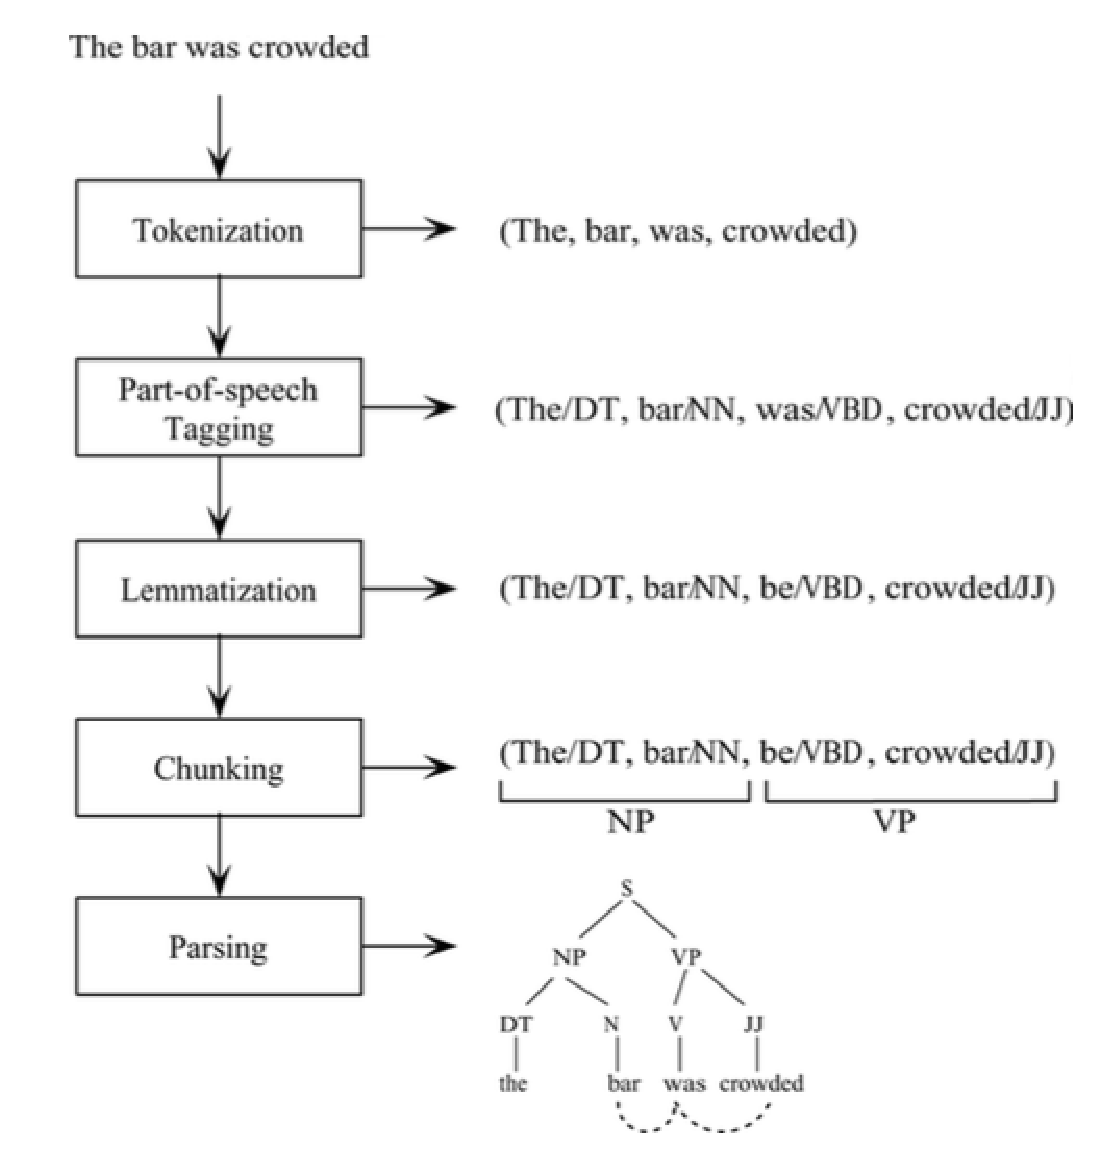
\includegraphics[scale=0.5]{figures/preprocess.eps}
\caption{Preprocess steps for formatting unstructured source}
\end{figure}

The resources for WSD can be broadly classified as shown in the figure \ref{fig:wsd_knowledge}. The thesauri, ontologies and machine readable dictionaries forms the structured resources of knowledge. Thesauri provides information about relationships between words. Ontologies give the specifications of concepts of specific domains of interest. Raw corpora, sense-annotated corpora and collocation resources forms the unstructured resources. Brown corpus with a balanced collection of million words and Wall street journal corpus with 30 million words are few examples of raw corpora. SemCor is the largest and most used sense-tagged corpus. There are multiple corpus which tags the senses of different languages. This can be used in machine translation. Collocation resources has the tendency to register the words that commonly occur with other words. This resources are mainly derived from web data. 

\subsection{Representation of Context}
\label{ssec:contextRepresentation}

\begin{figure}
\centering
\epsfig{figure=figures/preprocess.eps,width=.5\textwidth}
%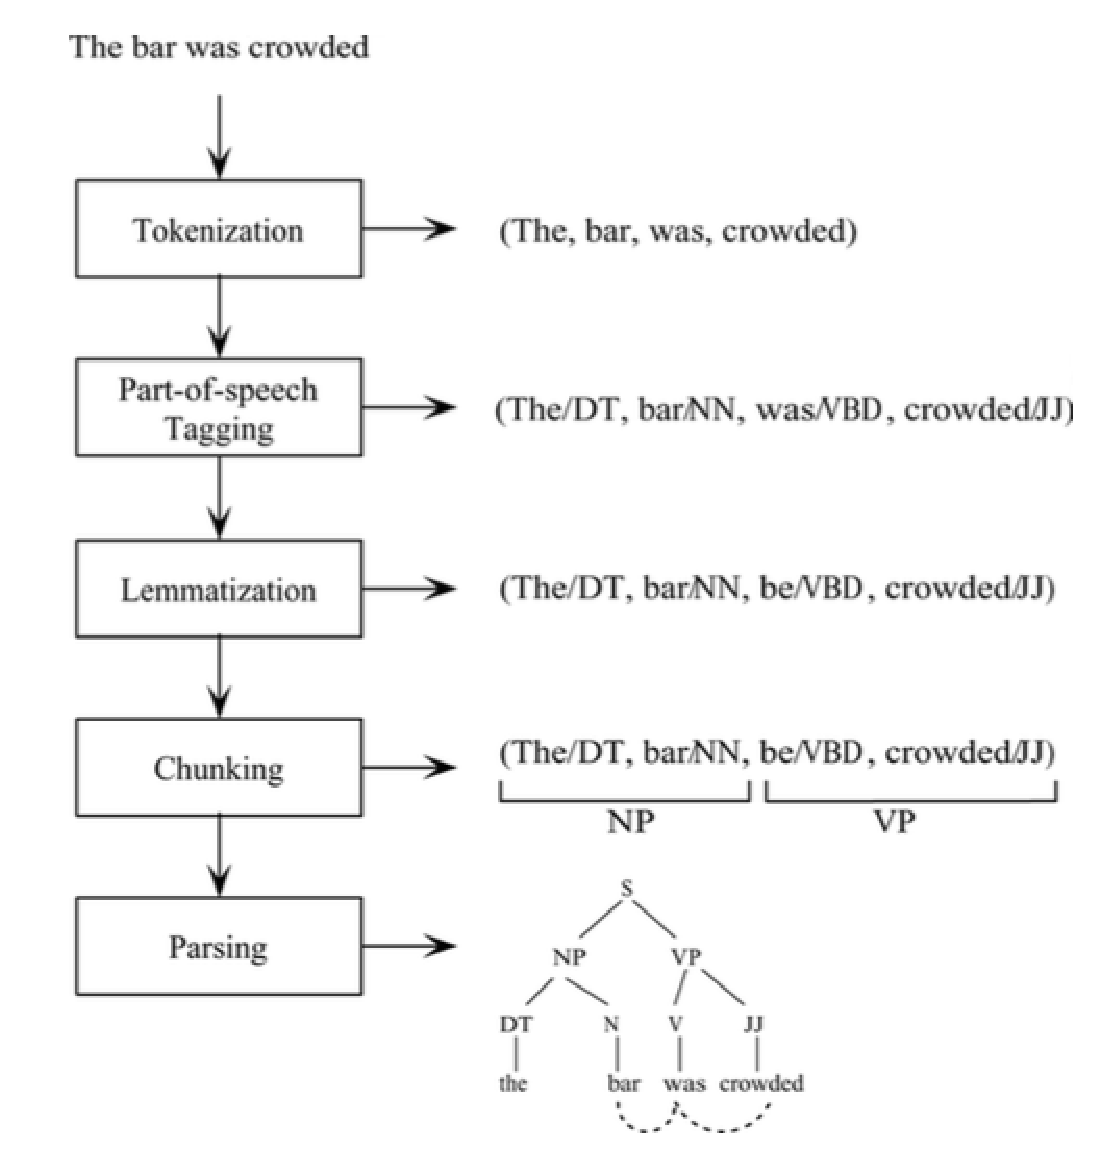
\includegraphics[scale=0.5]{figures/preprocess.eps}
\caption{CHANGE THE DIAGRAM}
\end{figure}

Unstructured source of information are pre-processed as displayed in the diagram. Tokenization splits up the text into set of tokens. Parts of speech tagging tags every word with its parts of speech usually noun, verb, determinant, 	and adjectives. Then lemmatization reduces the morphological variations to the basic form and chunking divides the text into syntactically correlated parts \cite{Jurafsky}. Finally parsing is used to identify the syntactic structure of the sentence. Usually a set of features are chosen to represent the context. The commonly used features are
\begin{itemize}
\item local features: represents the local context of the word usage based on the small number of words surrounding the target word.
\item topical features: is the complete opposite of local feature and describes the general topic of text or discourse.
\item syntactic features: explains the syntactic cues and argument head relations between the target word and other words within the same sentence. 
\item semantic features: explains the semantic representation based on the sense of words in the context. 
\end{itemize}

\subsection{Types of Classification}
\label{ssec:classificationTypes}

As we discussed already WSD can be considered as the classification task and three types of classification systems are:
\begin{itemize}
\item Supervised WSD
\item Unsupervised WSD
\item Semi-supervised WSD
\end{itemize}

\subsubsection{Supervised WSD}
\label{sssec:supervisedWSD}
This approach uses machine learning techniques to learn the class properties from labeled training data. It encodes the features of same class label together and check for the set of such features for the unlabeled data. It assigns the unlabeled data to the class that gives maximum similarity of features. Many approaches like 
\begin{itemize}
\item Decision list 
\item Decision tree
\item Naive Bayes approach
\item Neural network and
\item SVM 
\end{itemize} 
comes under the supervised classification of words and its senses. 
\begin{itemize}
\item {\bf Decision List: } A given word $w$ is represented as a feature vector and the 	decision list is prepared. A decision list is an ordered set created by a set of weighted "if-then-else" rules. The feature set (sense) with highest score for the input feature vector (word) of a test word is assigned to that sense (feature set). This is the basic way of scoring to assign a word with its senses list.
\begin{center}
\vspace{-0.5cm}
\begin{equation}
\hat{S}=argmax_{S_i} \in Senses_{D(w)}score(S_i)
\end{equation}
\end{center}
Many variations of this scoring is found in literature including probability, logarithms etc. 

\item {\bf Decision Trees: }are the predictive models used to represent the classification rules in a tree structure where the leaf nodes have the classified words. Each internal node represents
a test and each branch represents the outcome of the test. Based on the leaf nodes the predictions are made. The tree is based on the result of yes or no for the rules represented in the internal nodes. The empty leaf node indicates that no choice is made based on the rule in its parent node. 

\item{\bf Naive Bayes:} is the probabilistic approach based on the application of Bayes' theorem \cite{bayesClassifier}. It calculates the conditional probability of different senses of the word using
\begin{equation}
\hat{S}=argmax_{s_i \in Sensed_{D}(w)} P(S_i) \prod_{j=1}^{m}P(f_j|S_i)
\end{equation}
and the sense with maximum $\hat{S}$ is considered as the appropriate sense of the word.

\item {\bf Neural network:} is the computational model generated by the interconnection of artificially created nodes called neurons. It uses the features of input words to partition the contexts into non-overlapping sets corresponding to the desired outputs. The neuron producing the desired output has larger activation value than others. The sample neural network is shown in the Figure~\ref{fig:neuralNetwork}.
\begin{figure}[h!tb]
\centering
\epsfig{figure=figures/neuralNetwork.eps,width=.5\textwidth}
%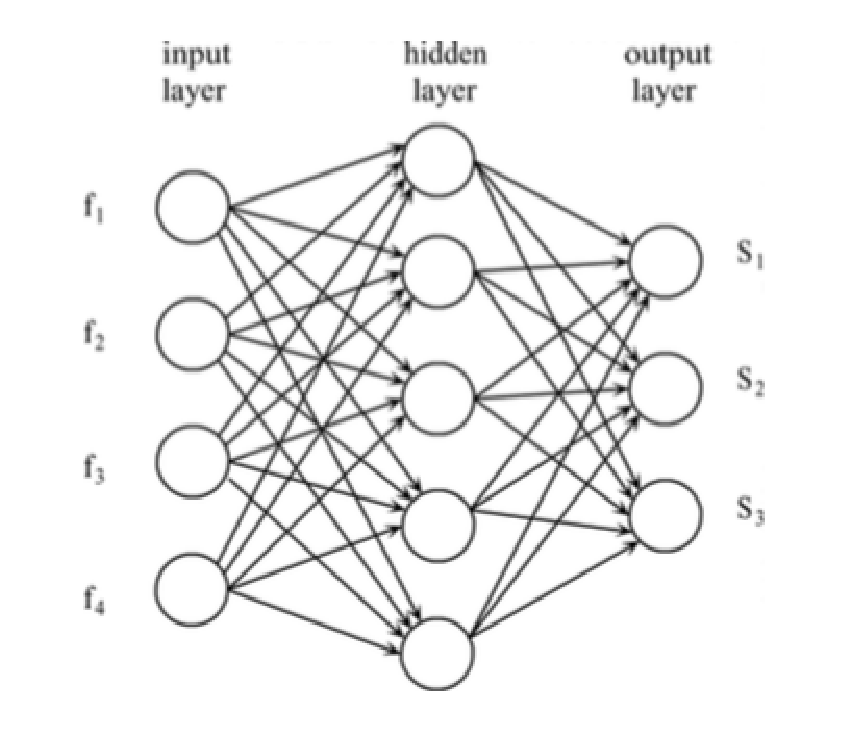
\includegraphics[scale=0.5]{figures/neuralNetwork.eps}
\caption{A sample neural network with input, hidden and output layers}
\label{fig:neuralNetwork}
\end{figure}

\item {\bf Support Vector Machines (SVM): } SVM is based on cover theorem which says on projecting the lower dimension to higher dimension leading to better classification of the data as shown in the Figure~\ref{fig:svmProjection}.
\begin{figure}[h!tb]
\centering
\epsfig{figure=figures/2dto3d.eps,width=.5\textwidth}
\caption{SVM projection from 2D to 3D}
\label{fig:svmProjection}
\end{figure}
The SVM aims at finding the separating hyperplane with margins. The data points that lies on the margin hyperplanes of the separating hyperplane are called support vectors. The separation is shown in the Figure~\ref{fig:supportVectors}.
\begin{figure}[h!tb]
\centering
\epsfig{figure=figures/svm.eps,width=.35\textwidth}
\caption{SVM with separating hyperplanes and support vectors}
\label{fig:supportVectors}
\end{figure}
\end{itemize}


\subsubsection{Unsupervised WSD}
\label{sssec:unsupervised}
This method completely uses the unlabeled data. It does not uses the manual tags to identify the sense of word in the context.  The main advantage of this method lies in the fact that it overcomes the knowledge acquisition bottleneck discussed in the beginning of the Section~\ref{sec:wsd}.  The basic idea of this process is that a word and its neighbor will have same sense. This is similar to K-nearest neighbor algorithms concept \cite{knn}. It is based mainly on the cluster allocation. It identifies the clusters instead of believing the assigned class. The different methods of unsupervised WSD is listed and explained one by one below.

\begin{itemize}
\item {\bf Context clustering:} A given sentence is taken as a bag of words and treated as context vector. Similarity between the two context vectors are mapped to the number of features. The similarity of the two vectors can be calculated by cosine similarity as shown in \ref{eqn:cosSim}.
\begin{center}
\vspace{-5mm}
\begin{equation}
sim(u,v)=\frac{u.v}{|u|.|v|}=\frac{\sum_{i=1}^{m}}{\sqrt{\sum_{i=1}{m}u_i^2 . \sum_{i=1}^{m}v_i^2}}
\end{equation}
\label{eqn:cosSim}
\end{center}

\begin{figure}
\centering
\epsfig{figure=figures/contextClustering.eps,width=.75\textwidth}
\caption{Figure (a) is an example of two vectors. Figure (b) is a context vector for stock, and the centroid of the vectors of word}
\label{fig:vectorSpace}
\end{figure}
As the number of words increases the set of vectors corresponding to the words goes to infinity. The context clustering results in the word vector matrix as shown below

\begin{equation}
\bordermatrix{~ & v_1 & v_2 & \cdots & v_n \cr
                  w_1 & 1 & 0 & \cdots & 1 \cr
                  w_2 & 0 & 1 & \cdots & 1 \cr
                  \vdots & \vdots &  \vdots & \cdots & \vdots \cr
                  w_n & 1 & 1 & \cdots & 1}
\end{equation}
Latent semantic analysis (LSA) is based on this context clustering.

\item {\bf Word clustering:} Word clustering is the clustering process between two words say $w_i$ and $w_j$. This clustering is a 3 step process. The first step is the $S-step$ where the similarity between the two words is calculated as $sim(w_i,w_j)$ where the information in the  feature vector. The second step is the $C-step$  determining the set of clusters for each word. This $C-step$ commits the word with each cluster. The last step is the $D-step$ known as discrimination step $w_i$ $\in$ $E$ the set of clusters. 

\item {\bf Co-occurrence graphs:} Let $G$ be the graph with $V$ vertices and $G$ edges. The words are the vertices and the co.occurrence syntactic relation are the edges. Let $w$ be the target or ambiguous word and $G_w$  is the local graph around $w$. The adjacency matrix has to be created and normalized to get the Markov chain. The markov clustering algorithm has two steps namely $E-step$ (Expectation step) and $I-step$ (Inflamation step). HyperLex is the hyper lexicon where the similarity between the two words $w_i$ and $w_j$  as 
\begin{equation}
w_{ij} = 1 -max { P(w_i | w_j),P(w_j |w_i)} \\
P(w_i | w_j) = \frac{freq_{ij}}{freq_j} \\
P(w_j | w_i) = \frac{freq_{ij}}{freq_i}
\end{equation}

Minimum spanning tree (MST) is another representation generated from the co.occurrence graph to remove the ambiguity in the graph. To generate MST first arrange the ascending weights such that the co.occurrence graphs order is preserved. 
\end{itemize}

\section{Semantic Relatedness}
\label{sec:sr}

TO estimate the similarity between a pair of words, semantic relatedness is used to identify something apart from the literal meaning of both the words. The set of possible synonyms for a word collected from external world knowledge is called as Synonym-set or simply {\bf synset}. Each synset is associated with a small description called as {\bf gloss}. Synsets are easy to encode because they are direct words. Synset is referred using ID's. Each synset is associated with a series of glosses. Preferable cardinality of synset to be greater than one. The main advantage of this is that we can have more words and context. The normal functional relations like symmetry, reflexive etc. The estimation of semantic relativeness between words is measured is determined by three different ways as given below.
\begin{itemize}
\item 	Wordnet-based
\item Distributional similarity based on corpora
\item Introspective distributional similarity 
\end{itemize}

\subsection{WordNet based method}
\label{ssec:wordNet}

Word sense disambiguity (WSD) is used to come -up with appropriate synsets for each word from the synset word. To find the relationship between synsets we use the taxanomy of wordnet. One way to do without WSD is find out all possible similarity for $w_i$ from the synset-word relationship. If the synsets of two words are more related, then the words are said to be related too. The measures of similarity between synsets can be measured in more than one ways. Two such methods are 
\begin{itemize}
\item Path-based measures
	\begin{itemize}
	\item Wu-Palmer Measure (WPM)
	\item Liu similarity measure 
	\end{itemize}
\item Information content based measures
\end{itemize}

\subsubsection{Path-based measures}
\label{sssec:pathBasedMeasure}
\begin{itemize}
\item {\bf Wu-Palmer Measures (WPM):} The sum of distance to the lowest common ancestor (LCA) in a tree structure with respect to two leaf nodes (word1 and word2) under consideration and the sum of the distance to the root as mentioned in the Equation 

\begin{center}
\begin{equation}
WPM=1-\frac{sum\;of\;the\;distance\;to\;LCA}{sum\;of\;the\;distance\;to\;the\;root}
\end{equation}
\label{eqn:wpm}
\end{center}

Bigger the WPM measure, the LCA measure is the similarity measure and it must be preferably higher and the root distance measures the distance which must be preferably lower \cite{wuPalmer}. The similarity between two classes C1 and C2 is measured by {\it Wu-Palmer similarity score} as

\begin{align*}
sim(C1,C2) &= \frac{2 \times N_{3}}{N_{1}+N_{2}+2N_{3}} \\
					&=\frac{N_{1}+N_{2}}{N_{1}+N_{2}+2N_{3}}
\end{align*} where $N_1, N_2$ are the number of links from $C1,C2$ to their most specific common superclass and $N_3$ a=is the number of links from the most specific common superclass to the root. 

\item {\bf Liu similarity measure:} 
\begin{center}
\begin{equation}
sim(C1,C2)=\frac{e^{\alpha L} e^{\beta H} - e^{- \beta H/} }{e^{\beta H} + e^{- \beta H/}}
\end{equation}
\end{center}
\end{itemize}
where $\alpha \geq 0, \beta \geq 0$ are constants, $L$ is the shortest path between $C_1, C_2$ and $H$ is the depth in taxonomy of the most specific common concepts in a non-linear function.

\subsubsection{Information theoretic based measure}
\label{sssec:informationBasedMeasure}

This method is proposed to overcome the disadvantages of the path-based measures discussed in Section \ref{sssec:pathBasedMeasure} like similar treatment for the words at same level and the skewness based on the tree structure. The tree is constructed manually and it may not reflect all world knowledge. This measure also uses LCA as

\begin{center}
\begin{equation}
IC(S_1,S_2)=log \left(  \frac{1}{P(LCA(S_1,S_2))}  \right)
\end{equation}
\end{center}

The denominator term is estimated based on the corpora. The disadvantage of this method is the word in search may not be ithere directly but many related synsets will be there. Such similar synsets are also needed to be considered to calculate the probability.

\subsection{Distribution similarity based on corpora}
\label{ssec:distSimilarityCorpora}
Wikipedia is a generic resource which explains the representation of knowledge and how the data related data are linked to it. The reference to one page may trigger many related memories leading to a search for the related topics. For example if we search for bishop it may lead to rook so that one may know that too. But both are related through a game named Chess. 

\subsubsection{Explicit semantic analysis}
\label{sssec:esa}
Explicit semantic analysis (ESA) is an analysis method used to identify or handle the distributional similarity based on corpora like Wikipedia. This analysis is based on {\it vector-space modeling} \cite{esa}. ESA is used for two tasks like
\begin{itemize}
\item Estimating relativeness  between two pieces of text
\item estimating relativeness between two words
\end{itemize}

Input texts are represented as weighted vectors of concepts called {\it interpretation vectors}. 
Semantic relatedness of texts are computed by comparing the vectors defined in the concepts space. The explicit meaning is intended to capture the concepts grounded in human cognition. The inputs are given in the form of plain text and the conventional classical algorithms are used to rank the concepts represented by the document. Each document is represented as a vector of words and conventional classification algorithms to rank the concepts represented by these documents. Each documents is assigned with a weight vector identified by the TFIDF discussed in Section \ref{sec:ir}. The vector space modeling of the words and its concepts will look very similar to the Figure \ref{fig:vectorSpace}.  The vector space model can be spanned either by word vectors as basis vectors or concept vectors as basis vectors.

Mapping of words from word space to concept space are done offline irrespective of query using inverted index. This mapping is working on the basis of information retrieval on classification data. If a single words leads to many vectors in concept space, take a centroid of all those vectors and use it as the equivalent of that word in the concept space. The input document is treated as a bag of words $( w_1, w_2, w_3, \cdots, w_n)$ and mapped to $( v_1, v_2 , v_3, \cdots , v_n)$. Let $k_j$ be the TFIDF values of concept $c_j$ then the page rank of each document is calculated according to this TFIDF. Relevance measure of a concept $c_j$ to the document is measured as the sum of products of $v_i$ and $k_j$. 

\subsection{Distribution (Introspective) Approach}
\label{ssec:introspectiveApproach}

Estimated semantic analysis has the potential to do dimensionality reduction. Similar to spell check application this too requires feature selection \cite{featureSelection}. Word-word relation gives the ability to compress the dimension and relate it to a cluster. The basic idea of this distributional approach is no external knowledge like wordNet or wikipedia etc. Minimum description length (MDL) has connection  with Bayesian classification/inferences. MDL is the information theoretic approach whereas the Bayesian classification is the probabilistic approach. MDL concentrates on minimizing the length of encoding. Bayesian classification will maximize the posterior. Sometimes during the training of models we will not concentrate on over training to avoid over-fitting problem. Decision trees are used to define hypothesis. FUlly grown decision tree is the over-fitting kind of problem while shallo decision tree has the risk of over-generalization. KL-Divergence is the asymmetric measure between two probability distributions. Here KLD is used to measure the  distributional similarity between two words. The KLD between two distribution P and Q are defined as in the equation given below.

\begin{center}
\begin{equation}
D_{KL}(P,Q) = \sum_{x}P(x)log \frac{P(x)}{Q(x)} 
\end{equation}
\end{center}

KLD gives expected number of bits to represent the samples from P using Q. This measure is based on entropy. Entropy is a measure of uncertainty and it is used to assign an item x to any one of the classes under consideration. For a subset with all examples belonging to one class has zero entropy. If number of examples belonging  to the positive and negative classes are same then the entropy will be 1. Usually entropy varies between 0 to 1. Entropy of a set S with (+,-) classes is given as

\begin{center}
\begin{equation}
H(S)==P_{+}log_2P_{+} - P_{-}log_2P_{-}
\end{equation}
\label{eqn:entropy}
\end{center}

Introspective measures are mainly based on orders of co-occurrence patterns. 
Let us consider two words A and B. If both occurs in same document . Then they are said to be in first order co-occurrence. If those words are connected through some other word say C in two different documents then A and B are said to be second order co.occurrences and so on. The semantic relatedness between words using co.occurrences of words is done if it is a weighted graph. Semantic relatedness is calculated as the sum of all co-occurrences between a pair of words. 

Let us assume a set of words forming a directed graph as shown in figure given below. If 'B' is used in definition of A,D,C the edges will be like as in graph. The word with more incoming edges will be the foundational word. Or, the words of ancient origin are considered as foundational words.The alternate way is to prefer topological sort using page rank algorithm which helps in calculating the age of acquisition of words in child knowledge. 

\section{Circularity Problem}
\label{sec:circularity}
{\it Documents are similar, if they have similar words. Words are similar if they occur in similar documents}. The previous sentence defines a problem of circularity. The problem where something is needed to define one thing and that one thing is needed to define that same thing. The circularity problem is seen everywhere in NLP applications like word sense disambiguation, page ranking, information retrieval, co.occurrence patterns etc. The circularity can be resolved by using any one of the machine learning techniques discussed in following subsections. 

\subsection{K-Means Algorithm}
\label{ssec:kmeans}
 K-means algorithm is the simplest clustering algorithm to cluster the data in unsupervised learning. This classifies the data point into clusters based on $apriori$. One the cluster centroids are given the data point will be assigned to each cluster and cluster centroid is changed iteratively based on the data points. In NLP, K-means clustering is used in term-document clustering. Say the documents are represented in the space spanned by the terms. Out of many documents $\vec{x}$ in the space, it can be represented by the centroid $\vec{\mu}$ of the document cluster $\omega$ as
 \begin{center}
 \begin{equation}
 \vec{\mu}(\omega)=\frac{1}{|\omega |}\sum_{\vec{x}\in \omega}{\vec{x}}
 \end{equation}
 \label{eqn:kmeans_mu}
 \end{center}
  
To achieve this the documents to be compared are assumed to be length normalized. Ideally the clusters must not overlap to each other. The process can be completed after fixed number of iterations or until there is no much difference between the clusters formed by subsequent iterations. Since there is only a finite set of possible clusterings, a monotonically decreasing algorithm will eventually arrive at a (local) minimum. 

\begin{algorithm}[h!tb]
\caption{K-means algorithm}
\label{algo:kmeans}
\begin{algorithmic}[1]

\STATE \COMMENT{\textbf{Input:} Documents in term space or terms in document space\\
\textbf{Output:} Clusters and cluster centroids}
\STATE Randomly initialize $k$ clusters.
\STATE Calculate distance between each data points and all the cluster centroids
\STATE Assign the data point to the closest cluster
\STATE Recalculate the mean r centroid of each cluster with assigned data points
\STATE Repeat the steps from 2 to 4 until termination condition.
\end{algorithmic}
\end{algorithm}

{\bf Advantages:} Robust, simple, relatively efficient. Effective when the data points are distinct and well separated. 

{\bf Disadvantages:} We have ti determine the number of clusters or centroids in prior. This has to be related with the actual classes or varities of data. Else the resulting clusters may not be appropriate. Fails to handle noisy data, outliers and non-linear data. 

\subsection{Expectation Maximization Algorithm}
\label{ssec:emAlgorithm}

EM algorithm is used to handle the circularity problem. EM algorithm is used as a classifier. The EM algorithm is applied on GMMs. The weights of each Gaussian mixture component is calculated along with the mean and the variance. The mixture weights and parameters are estimated in Estimation step (E-step) and the parameters are used to maximize the posterior probability in Maximization (M-step).
	
EM algorithm has a wide application range in the statistics of natural language process, such as the forward-backward algorithm in HMM, the inside- outside algorithm in PCFG, EM clustering algorithm and no supervision semantic disambiguation algorithm, which are the specific applications of EM algorithm for parameter estimation problems.

EM might look like a heuristic method. However, as we show now, it has a rigorous foundation: EM is guaranteed to find a local optimum of data log likelihood.  EM is an iterative procedure to maximize the marginal log likelihood $l(\theta)$. 

{\bf Step 1:} The step 1 of EM algorithm (E step) is to find logarithm likelihood function $log p(X, Y | \theta )$, while given observation data set X and the current parameter set $\theta (i-1)$, the expectation value about unknown data set Y is the value to calculate the next expression: $ Q( \theta , \theta (i-1)) = E [log p(X,Y | \theta(i-1))]$ , here into $\theta$ is the new parameter set after optimization and makes the value of function Q increasing with the new parameter.

{\bf Step 2:} The step 2 (M step) of EM algorithm is to maximize expectation value of part 1, that is next expression $ \theta (i) = argmax_Q (\theta , \theta (i-1))$, this $\theta$ two steps constantly iterates, each iteration will ensure to increase the logarithm likelihood function values and ensure that likelihood function converges to a local maximum value point.

\subsection{Page ranking}
\label{ssec:pageRank}

The Google search engine uses Page Rank algorithm to exploit the linked structure of the web. This page rank helps in computing the global importance scores that can be used to influence the ranking of search results. The rapid growth in web increased the demand for greater flexibility in ranking and page rank algorithm is proven to be effective in achieving this. Ideally each user should be able to define his own notion of importance for every query posed by him. 

In principle personalized page ranking algorithm can be effective to achieve this. But it requires naive implementation and computing resources far beyond the realm of feasibility. Page rank assigns score to the web pages. A page is important if it is pointed-to by several important pages. Based on the number of link pointing a page and from who the reference is coming the weightage of a page will be altered. 


From the diagram $P_4 = P_1 + p_2 + P_3$ where P is a vector that only gets scaled or stretched but it does not rotate when the operator acts on it.  Page rank has the solution to the circularity problem but not the optimal one. PCA can handle circularity with optimal solution. 

\subsection{Singular Value Decomposition}
\label{ssec:svd}

Singular value decomposition (SVD) is used to solve the problem of circularity by using the covariance matrix as a feature matrix. SVD follows matrix diagonalization theorem splits a matrix into three where the middle one is the diagonal matrix with the eigen values and the other matrices has eigen vectors in it. If a matrix A has a matrix of eigenvectors P that is not invertible  then  A does not have an eigen decomposition. However, if A is an $m \times n$ real matrix with $ m > n$, then A can be written using a so-called singular value decomposition of the form $A=UDV^(T)$. 

Singular values are the square root of eigenvalues. Eigenvectors computed from the covariance matrix represents the maximum energy varying directions and eigenvalues gives the magnitude of these vectors. If the eigenvalues are unique and independent the eigenvectors will be linearly independent of each other. If the covariance matrix is symmetric and positive definite the eigenvectors will be orthogonal to each other. Note that there are several conflicting notational conventions in use in the literature. U to be an $m \times n$ matrix, D as $n \times n$, and V as $n \times n$. However, the Wolfram Language defines U as an $m \times m$, D as $ m \times n$, and V as $ n \times n$. In both systems, U and V have orthogonal columns so that  $U^(T)U=I$ and $V^(T)V=I$. In NLP SVD is performed on word-word covariance matrix obtained by the distribution of words over the documents. The words are the linear combination of the eigen values of the word-word covariance matrix. 

\hspace{-5mm}
\begin{minipage}{0.35\textwidth}
\centering
\begin{equation*}
\bordermatrix{~ & w_1 & w_2 & \cdots & w_{|V|} \cr
                  D_1 & ... & ... & \cdots & ... \cr
                  D_2 & ... & ... & \cdots & ... \cr
                  \vdots & \vdots &  \vdots & \cdots & \vdots \cr
                  D_n & ... & ... & \cdots & ...} 
\end{equation*}
\small{a) Term Document Matrix}
\end{minipage}%
\begin{minipage}{0.35\textwidth}
\centering
\begin{equation*}
\bordermatrix{~ & w_1 & w_2 & \cdots & w_{|V|} \cr
                  w_1 & ... & ... & \cdots & ... \cr
                  w_2 & ... & ... & \cdots & ... \cr
                  \vdots & \vdots &  \vdots & \cdots & \vdots \cr
                  w_n & ... & ... & \cdots & ...} 
\end{equation*}
\small{b) Covariance Matrix}
\end{minipage}%
\begin{minipage}{0.35\textwidth}
\begin{equation*}
                  \bordermatrix{~ & e_1 & e_2 & \cdots & e_{|V|} \cr
                  D_1 & ... & ... & \cdots & ... \cr
                  D_2 & ... & ... & \cdots & ... \cr
                  \vdots & \vdots &  \vdots & \cdots & \vdots \cr
                  D_n & ... & ... & \cdots & ...} 
\end{equation*}
\small{c) EigenVector Document Matrix}
\end{minipage}

$e_i$ is the eigen vector with the linear combination of words and hence it can be termed as $eigen documents$ . Now we get 3 more documents which are not in document collection. Now we have $D_n+3$ documents along with the initial documents. These documents can also be represented along with the initial document $(D_i)$.

\subsection{Principle Component Analysis}
\label{ssec:pca}
Principle component analysis (PCA) also known as {\textit unimodal factor analysis (UFA)}. 	PCA performs orthogonal transformation to convert a set of observations of possibly correlated variables into a set of values of linearly uncorrelated variables called principle components. The number of principle components are less than or equal to number of original variables. This transformation is defined in such a way that the first principal component has the largest possible  variance and each succeeding component in turn has the highest variance possible under the constraint that it is orthogonal to the preceding components. The resulting vectors are an uncorrelated orthogonal basis set. The principal components are orthogonal because they are the eigenvectors of the covariance matrix, which is symmetric. PCA is sensitive to the relative scaling of the original variables.

\begin{algorithm}[h!tb]
\caption{Principle component analysis}
\label{algo:pca}
\begin{algorithmic}[1]
\STATE \COMMENT{\textbf{Input:} Data points / terms / words\\
\textbf{Output:} Principle components and its directions}
\STATE Subtract mean of the data from all the data points
\STATE Calculate the covariance matrix
\STATE Calculate eigenvalues and eigen vectors of the covariance matrix
\STATE Choosing components and forming the feature vector
\end{algorithmic}
\end{algorithm}


\subsection{Latent Semantic Analysis}
\label{ssec:LSA}

Matrix diagonalization theorem applied on a symmetric covariance matrix gives eigenvectors will be orthogonal in nature to each other. sometimes orthogonality is the essential property. 
Latent Semantic Analysis (LSA) is a theory and method for extracting and representing the contextual-usage meaning of words by statistical computations applied to a large corpus of text. The underlying idea is that the aggregate of all the word contexts in which a given word does and does not appear provides a set of mutual constraints that largely determines the similarity of meaning of words and sets of words to each other. The adequacy of LSA’s reflection of human knowledge has been established in a variety of ways. Word and passage meaning representations derived by LSA have been found capable of simulating a variety of human cognitive phenomena, ranging from developmental acquisition of recognition vocabulary to word-categorization, sentence-word semantic priming, discourse comprehension, and judgments of essay quality.


LSA can be construed in two ways: (1) simply as a practical expedient for obtaining approximate estimates of the contextual usage substitutability of words in larger text segments, and of the kinds of as yet incompletely specified meaning similarities among words and text segments that such relations may reflect, or (2) as a model of the computational processes and representations underlying substantial portions of the acquisition and utilization of knowledge. LSA represents the meaning of a word as a kind of average of the meaning of all the passages in which it appears, and the meaning of a passage as a kind of average of the meaning of all the words it contains. LSA's ability to simultaneously derive representations of these two interrelated kinds of meaning depends on an aspect of its mathematical machinery that is its second important property. LSA assumes that the choice of dimensionality in which all of the local word- context relations are simultaneously represented can be of great importance.

\subsubsection{LSA Application}
\label{sssec:lsaAppln}
Cross language retrieval and document preparation are the major applications of LSA. 
Cross language retrieval will have same text in both language will give us the difference between the languages after proper model training through LSA. To make a document of sentences and there translation and LSA will come up with interesting pattern of co.occurrences. 

\section{Parsing}
\label{sec:parsing}
Since the human language is highly recursive and ambiguous, syntax are needed. Parsing is the process of analysing the syntax and determining the meaning. The man goals are to get the structure to validate the sentence meaning, to identify the parts of speech, to co-reference resolution within the sentence, and to get the meaning of the sentence. Inducing grammar rules in a language is a big problem. If we downsize the problem to some basic set of rules along with the probabilities alongside it. EM algorithm is used to learn the probabilities associated with rules. 

\begin{figure}
		\centering
		\epsfig{figure=figures/parseTree.eps,width=.7\textwidth}
		\caption{Example of a parse tree}
		\label{fig:parseTree}
\end{figure}

The advantage of parts of speech tagging is "re-usability" but it has its limitations. The context free grammars can be used to implement parsers, and discuss chart parsing, which allows efficient processing of strings containing a high degree of ambiguity. The idea of a context-free grammar (CFG) should be familiar from formal language theory. A CFG has four compo- nents, described here as they apply to grammars of natural languages:
\begin{itemize}
\item a set of non-terminal symbols (e.g., S, VP), conventionally written in uppercase;
\item a set of terminal symbols (i.e., the words), conventionally written in lowercase;
\item  a set of rules (productions), where the left hand side (the mother) is a single non-terminal and the right hand side is a sequence of one or more non-terminal or terminal symbols (the daughters);
\item  a start symbol, conventionally S, which is a member of the set of non-terminal symbols.
\end{itemize}

\subsection{Classical Parser}
\label{ssec:classicalParser}
Classical parsing is the process of just parsing the input sentence based on the formulated general grammars. Generally this is classified into {\it top-down parsing} and {\it bottom-up parsing}. 
\begin{itemize}
\item {\bf Top down parsing:}
A top-down parser starts with the root of the parse tree. It is labeled with the start symbol or the goal symbol of the grammar. TO build the parse tree, it repeats the following steps until the leaves of the parse tree matches the input string.
\begin{itemize}
\item At a node labeled A, select s production with A on its left-hand-side and for each symbol on its right-hand-side, construct the appropriate child.
\item When a terminal is added to the leaf that does not match the input string backtrack.
\item Find the next node to be expanded. It must have a label in non-terminal.
\end{itemize} The main key in this top-down parsing is to select the right production in Step - 1.
\item {\bf Bottom up parsing:} Bottom up parsing has same grammar and the procedures. But it starts at the leaves and grow in-wards. Starting in a valid state for legal first token is the first step in bottom up parsing. As an input is consumed, the state is changes to encode the possibilities. That is to recognize the valid preferences. Bottom up parsing uses a stack data structure to store both state and sentential forms.
\end{itemize}

\subsection{Parse Generation}
\label{ssec:parseGeneration}
Classical parse trees are used to check the validity of a existing or formulated grammar \cite{Charniak97}. Generating the parse tree automatically based on the given grammar is called as parse generation and it can be done in two ways namely  {\it constituency parsing} and {\it dependency parsing}.
\begin{figure}[h!tb]
\centering
		\epsfig{figure=figures/constituency.eps,width=.7\textwidth}
		\caption{Constituency and dependency parsing}
		\label{fig:constituencyParser}
\end{figure}


A constituency parse tree breaks a text into sub-phrases. Non-terminals in the tree are types of phrases, the terminals are the words in the sentence, and the edges are unlabeled. For a simple sentence "We are trying to understand the difference", a constituency parsing and dependency parsing would look like as in the Figure~\ref{fig:constituencyParser}. A dependency parse connects words according to their relationships. Each vertex in the tree represents a word, child nodes are words that are dependent on the parent, and edges are labeled by the relationship. Out of these two parsers the parser which may take us close ot the assigned goal has to be chosen.

\subsection{Probabilistic parser}
\label{ssec:probParsing}
Probabilistic parsing is using dynamic programming algorithms to compute the most likely parse(s) of a given sentence, given a statistical model of the syntactic structure of a language. As we see in previous chapter same grammar may lead to more than one parser. The problem of this ambiguity and chaos can be get-rid by probabilistic context free grammars. Probabilistic grammars are used to
\begin{itemize}
\item determine the sentence and 
\item choose the speedier parser
\end{itemize}

\hspace{-5mm}
\begin{figure}
\begin{minipage}{0.45\textwidth}
\centering
\epsfig{figure=figures/pcfg1.eps,width=.7\textwidth}
\end{minipage}%
\begin{minipage}{0.45\textwidth}
\centering
\epsfig{figure=figures/pcfg-2.eps,width=.7\textwidth}
\end{minipage}
\caption{Probabilistic CFG}
\end{figure}


{\bf Tree bank:} The pure grammar induction approaches tend not to produce the parse trees that people want. A fairly obvious approach to this problem is to give a learning tool with some examples of the kinds of parse trees that are wanted. A collection of such example parses is referred to as "tree bank". Because of the usefulness of collections of correctly-parsed tree banks, but by far the most widely used one, reflecting both its size and readily  available status {\it Penn Treebank"} is used more commonly.

\section{Machine Translation}
\label{sec:machineTrans}
Machine Translation (MT) is the task of automatically converting one natural language into another, preserving the meaning of the input text, and producing fluent text in the output language.  The ideal aim of machine translation systems is to produce the best possible translation without human assistance. Basically every machine translation system requires programs for translation and automated dictionaries and grammars to support translation.

Machine translation is handled with the assumption that while transferring the data over a noisy channel it may get corrupted or altered. To get back the original message from the received message we need to understand the channel features and the noise in it. The same scenario is used here where the analogy of channel model maps to the language model here. In figure~\ref{fig:NosiyChannel}  {\it{e}} represents English which acts as a target language and {\it f} represents French which is our source language. 

\begin{figure}[h!tb]
\centering
\epsfig{figure=figures/mt.eps,width=.5\textwidth}
\caption{Noisy channel model of Machine translation}
\label{fig:NosiyChannel}
\end{figure}

Using Bayes theorem we have to identify 
\begin{center}
\begin{equation}
P(e|f)=\frac{P(e).P(f|e)}{	P(f)}
\end{equation}
\label{eqn:mtBayes}
\end{center}

and the best Engllish translation for the French sentence in hand is obtained by $\hat{e}=argmax_e P(e)P(f|e)$. Now the translation problem is reduced to a language problem of identifying the $Prior$ $P(e)$ and a $translation$ task of identifying $P(f|e)$. IBM model is used to identify the translation task alone whereas the language model can be built using $Markovian$ based {\it Hidden-Markov-Model}. 

Statistical machine translation handles complete data directly and the incomplete data through EM algorithm (Section~\ref{ssec:emAlgorithm}). Word-pair alignments gives rise to the sentence pairs. The sentence pairs do not have the information of the word-pair alignments given rise to them.
In all cases, the translation probability $P(f|e)$ is seen as the sum on all alignments of the conditional probabilities $P(f,a|e)$, where a is an alignment between the French and the English sentences:
\begin{center}
\begin{equation}
P(f|e) = \sum_a P(f,a|e)
\end{equation}
\label{eqn:transitionProb}
\end{center} and the conditional probability $P(f,a|e)$ is defined as 
\begin{center}
\begin{equation}
P(f,a|e)=P(m|e) \prod_{j=1}^{m} P( a_{1}^{j-1},f_{1}^{j-1},m,e) . P(f_{j} | a_{1}^{j}, f_{1}^{j-1},m,e)
\end{equation}
\end{center}

The best alignment is calculated as 
\begin{equation}
\hat{a}=argmax_aP(a,f|e)
\end{equation}

The translation model informs us on what sentences are good translations, while the language model ensures that these sentences are well-formed. By combining these models, we thus get better results than if we were to look directly for the sentence that maximizes $P(e|f)$.

\subsection{IBM Model 3}
\label{ssec:ibmModel3}
IBM Model 3 is an example for statistical machine translation. 

\hspace{-5mm}
\begin{figure}[h!tb]
\begin{minipage}{0.45\textwidth}
\centering
\epsfig{figure=figures/MT-example.eps,width=.8\textwidth}
\end{minipage}%
\begin{minipage}{0.45\textwidth}
\centering
\epsfig{figure=figures/MT-example2.eps,width=.8\textwidth}
\end{minipage}
\caption{An example for machine translation}
\label{fig:mtExample}
\end{figure}

IBM model 3 is a generative model which calculated the best alignment and translation probability as discussed previously. The three important parameters needed for this model are
\begin{itemize}
\item Fertility parameter : $n(\phi_j |e _j)$
\item Translation parameter : $t(f_i | e_{aj}$
\item Distortion parameter : $d(f_{pos}=i | e_{pos} = j, I,J)$ 
\end{itemize}
where I and J are the total words presents in the English and French sentences respectively and $i,j$ refers the words in the respective languages. The transformation of English sentence to French is shown in the Figure~\ref{fig:mtExample2}. Fertility parameter explains whether any word is replicated/deleted during the transformation and the translate parameter calculates the translation probability as discussed earlier. The distortion parameter measures the amount of re-ordering of the translated words needed to get a proper translated sentence.

\begin{figure}[h!tb]
\centering
\epsfig{figure=figures/mt_eg3.eps,width=\textwidth}
\caption{An transformation of English to French by the IBM Model 3 with  parameter set}
\label{fig:mtExample2}
\end{figure}

Knowing the parameter values the probability can be calculated easily for sentence pair. If the parameters are unknown, IBM model 3 is tough to use. So we have to align words using IBM model 1 to get the best alignment and  the parameters are learned using the same model. Then transition models are built using IBM model 2 and the final parameter set is used as the seed to IBM model 3 to calculate the probability.
\clearpage 

\begin{center}
\huge{Chapter 4}
\end{center} 

\section{Choosing the words in computer-generated weather forecasts}
\label{sec:introPaper}

Weather forecasts and daily weather reports are inevitable needs in our day-to-day life to know the climatic changes. Satellite images are the source of the weather reports. These satellite images can be interpreted only by the experts. Their interpretation are so crisp and too technical for the common people to understand. Transferring the technical information listed by the weather experts from the satellite images to the understandable text format can be done by employing humans for the task. The major problem with this is the inconsistent and ambiguous way of an individual in representing the content. This can be avoided by using an automated system to do the translation of information to the complete report.  

The humans have lot of ambiguity in understanding the things and there is no commonality between the understanding of two different persons. The color referred as "pink" by two persons may differ even in same lighting and with same visual perception capacity. This difference is termed as "idiolect differences" which raises an important question in implementing the computer based NLG system. The major problem due to the idiolect differences is "{\it {How does the text produced by the system in English (or other human languages) from non-linguistic input data ensures that the texts they produce are correctly interpreted by their readers?}"}.

This can be ensured by a common set of rules that are needed to be followed in choosing the words and phrasing the sentences and the resultant must be consistent and understandable to all type of people without any ambiguity. In \cite{forecast}, an automated weather report generator named SUMTIME-MOUSAM is discussed elaborately. SUMTIME-MOUSAM is the text-generator based on NLG concepts  voted as the best choice by users than the human-authored texts.

\subsection{Stages of text generation}
\label{ssec:stages}
SUMTIME-MOUSAM  is generated after 3 different stages of detailed analysis of the content to be translated and the content to be presented in the generated weather-reports. The three important stages are
\begin{itemize}
\item Document planning
\item Micro-planning and
\item Surface realization
\end{itemize}

{\bf Document planning: } decides on what content to be included and in the structure of that content in the report.  Mainly how the numeric information are going to be communicated as the text. A linear segmentation algorithm is used for this purpose which uses the pragmatic analysis of appropriate content for a weather forecast report. The structure of the report will be based on a human understandable schema or template on which the transcribed numerical information are included to make it readable and understandable.

{\bf Micro-planning: } plans how subtle the content and structure must be expressed linguistically. 	This step uses the NLP concepts like {\it lexicalisation, aggregation and expression generation}. {\it Lexicalization} determines which words are to be used to represent the information and {\it aggrgation} decides how to distribute the information across the sentences. And the last task of expression generation deals with the problem of referring back the entities introduced in the generated text.

{\bf Surface realization:} This phase generates the actual text according to the decisions made in previous stages. The key problem in this phase is to generate the special rules to generate the text in the weather sub-language called "weatherese" instead of conventional English. 

\subsection{Word choice}
\label{ssec:wordChoice}

Human forecasters usually use their own choice of words and lexical rules. When it comes to automatic method with common representation of texts, the possible problems are explained with  few examples. 

\begin{figure}[h!tb]
\centering
\epsfig{figure=figures/weatherData.eps,width=\textwidth}
\caption{Part of an input data set from SumTime-Mousam}
\label{fig:weatherData}
\end{figure}

Consider the table represented as the Figures~\ref{fig:weatherReport} generated from the information shown in the Figure~\ref{fig:weatherData}. Each sentence in Figure~\ref{fig:weatherReport} leads to a serious number of questions like 
\begin{itemize}
\item Should the direction "West" be expressed as W or W’LY?
\item Should the speed 8 knots be expressed as 8 or 08?
\item Should the verb "backing" or "becoming" be used to describe the change in wind direction?
\item Should the time pharse "by evening", "by late evening", or "by midnight" be used to express the
time 0000?
\end{itemize}  

\begin{figure}[h!tb]
\centering
\epsfig{figure=figures/weatherReport.eps,width=\textwidth}
\caption{Extract from forecast generated by SumTime-Mousam, from the input data set partially shown in Figure~\ref{fig:weatherData}. }
\label{fig:weatherReport}
\end{figure}

TO resolve this chaos, humongous human written forecast data are collected and analyzed. This analysis leads to a interesting observation that the data-to-text mapping depends on contextual factors like
\begin{itemize}
\item Preferences of individual writer and 
\item Linguistic context
\end{itemize}

Preferences of individual writer refers to the usage of different words by different persons to represent same chunk of data. The linguistic content represents the choice of word is influenced by linguistic factors such as the position of a word in a sentence.

\subsection{Choice of time phrases}
\label{ssec:phraseChoice}
A set of rules are needed to express which time phrase should be used in a weather forecast to communicate a numerical time from the input data file. This is done by an algorithm which first learns the way of representation from the human-forecaster' s text and then uses that to generate the rules. This analysis is done on the aligned corpus, where the content of the report as well as the phrases used by the forecasters in that content are aligned like a parallel corpus. The aligned corpus is generated from the normal data as follows.
\begin{itemize}
\item All similar statements that covers a period of 24 hours or less is collected
\item These statements are parsed and the linguistic structure of the wind statements are tuned.
\item Each phrase from the corpus corresponding to those time formats are aligned to the tuned linguistic structure. 
\end{itemize}
Tests on time phrases with unambiguous meanings (such as by midday) suggested that the alignment process was 86\% accurate.

\subsection{Classifier Analysis}
\label{ssec:classifyAnalysis}

Once the alignments are done, the next problem of what to choose when pops up? A classifier can handle this issue by tagging each scenario with certain probabilities to the possibilities in the database. The machine learning algorithms are used to learn classifiers which predicted which time phrase would be used in wind phrases extracted from the corpus. The classifier was trained only on wind phrases which had been successfully aligned with the data file. Similar to wind features, different features can also be aligned and the classifiers are trained to meet the end-users requirement. The other set of features that can be used are
\begin{itemize}
\item semantic features: information from the data file, such as the actual wind speed and direction
\item author feature: which forecaster wrote the text;
\item collocation features: the preceding and subsequent words in the text
\item repetition feature: the previous word of this type (time phrase) in the text
\item surface features: the length and position in the sentence of the phrase 
\item temporal features: when the forecast was issued, and how far in the future the prediction was from the forecast issue date.
\end{itemize}

\subsection{Summary}
\label{ssec:paperSummary}

People considerably vary with the usage of words as well as in the interpretation of words. Since we have crude understanding of our own language this variations do not affect the understanding. But when it comes to the system, what people mean and think with every word has to be represented clearly.
SUMTIME-MOUSAM, produced texts avoided the words which only occurred in one idiolect, and words whose meanings varied in different idiolects. But despite these flaws, human subjects still considered SUMTIME- MOUSAM’s texts to be more appropriate than human-written texts. It is possible to prepare the more generic report as well as the more idiolect specific reports. The texts generated by the NLG systems are more unambiguous and cheaper compared to the text reports produced by the human writers.
%%%%%%%%%%%%%%%%%%%%%%%%%%%%%%%%%%%%%%%%%%%%%%
%%                                          %%
%% Backmatter begins here                   %%
%%                                          %%
%%%%%%%%%%%%%%%%%%%%%%%%%%%%%%%%%%%%%%%%%%%%%%

\begin{backmatter}

\section*{Acknowledgements}
 I sincerely acknowledge to Prof. Sutanu Chakraborti for teaching us the concepts of NLP and guiding us in a righteous way to develop the subject knowledge that we acquire through the NLP classes. The cited articles and web-pages are acknowledged by referring them in reference section. 
%%%%%%%%%%%%%%%%%%%%%%%%%%%%%%%%%%%%%%%%%%%%%%%%%%%%%%%%%%%%%
%%                  The Bibliography                       %%
%%                                                         %%
%%  Bmc_mathpys.bst  will be used to                       %%
%%  create a .BBL file for submission.                     %%
%%  After submission of the .TEX file,                     %%
%%  you will be prompted to submit your .BBL file.         %%
%%                                                         %%
%%                                                         %%
%%  Note that the displayed Bibliography will not          %%
%%  necessarily be rendered by Latex exactly as specified  %%
%%  in the online Instructions for Authors.                %%
%%                                                         %%
%%%%%%%%%%%%%%%%%%%%%%%%%%%%%%%%%%%%%%%%%%%%%%%%%%%%%%%%%%%%%

\newpage 
\bibliographystyle{bmc-mathphys} % Style BST file (bmc-mathphys, vancouver, spbasic).
\bibliography{bmc_article}      % Bibliography file (usually '*.bib' )
\end{backmatter}


\end{document}
